\documentclass[a4paper,12pt]{article}
\usepackage[utf8]{inputenc}
\usepackage{polyglossia}
\setmainlanguage{spanish}
\usepackage{pythonhighlight}
\usepackage{multirow}
\usepackage{graphicx}
\usepackage{amsmath}
\usepackage[bookmarks = true, colorlinks=true, linkcolor = black, citecolor = black, menucolor = black, urlcolor = black]{hyperref}
%\usepackage[spanish,activeacute]{babel}
\usepackage{lmodern}
\usepackage{listings}
\usepackage{adjustbox}
\usepackage{float}
\renewcommand{\baselinestretch}{1} % Interlineado. 1 es estandar
\usepackage[T1]{fontenc}
\usepackage[square,sort,comma,numbers]{natbib}
\usepackage{mathtools}
\usepackage{fancyhdr}
\fancyhead[R]{2020}\fancyhead[L]{UNC - FCEFyN} \fancyfoot[C]{\thepage}
\pagestyle{fancy}
\usepackage[numbered]{bookmark} % Para que figure las secciones en el PDF
\graphicspath{ {img/} }

\begin{document}

\begin{titlepage}
	
	{\scshape\LARGE Universidad Nacional de Córdoba \par}
	%\vspace{1cm}
	{\Large Facultad de Ciencias Exactas, Físicas y Naturales \par}
	\vspace{0.5cm}
	\centering
	
\includegraphics[width=0.5\textwidth]{unc.png}
	\par\vspace{0.5cm}
	\vspace{0.5cm}
	{\scshape\Large Proyecto Final Integrador\par}
	\vspace{1.5cm}
	{\large\bfseries ``Predicción de cantidad de defectos graves en vehículos utilitarios en planta automotriz'' \par}
	\vspace{1.5cm}
	{\Large\bfseries Gerardo A. Collante\par}
	
	\vfill
	\textbf{Supervisor}\par
	Dr. Ing.~Orlando \textsc{Micolini}

	\vfill

% Bottom of the page
	{\large \today\par}
\end{titlepage}

\tableofcontents

\clearpage

\section{Motivación}

El \textit{machine learning} se ha erigido como un campo más en el mundo de las tecnologías de la información, sumado a su vertiginoso crecimiento y amparado bajo la constante mejora del \textit{hardware} ha hecho que su popularidad se dispare.

Más allá del todo el \textit{marketing} que envuelve a la tecnología, es innegable que los años venideros y mejoras en todos los campos serán en gran parte a la IA. Por tanto en búsqueda de mejorar profesionalmente emprendí este proyecto para a través de la práctica y la teoría obtener las herramientas necesarias para poder aspirar a un puesto como ingeniero de inteligencia artificial una vez finalizada mi etapa universitaria.

\clearpage

\section{Objetivo}

Se desea realizar un modelo de \textit{machine learning} capaz de predecir la cantidad de defectos graves utilizando como datos de entrada los defectos anteriores (de menor gravedad usualmente) considerando una ventana de tiempo a determinar.

En funcionamiento es muy similar a lo que se conoce como \textit{forecasting}, utilizado generalmente en la predicción del clima.

\clearpage

\section{Clasificación de modelos de inteligencia artificial}

Hagamos algunas definiciones para ponernos en contexto del campo sobre el cual este proyecto integrador será desarrollado.

\subsection{Inteligencia Artificial}

\begin{quote}
  La \textit{Inteligencia Artificial (Artificial Intelligence)} se define como el estudio de los "agentes inteligentes", i.e. cualquier dispositivo que perciba su entorno y tome medidas que maximicen sus posibilidades de lograr con éxito sus objetivos.
  
  \hfill \citet{poole1998}
\end{quote}

Esta definición nos da la idea de que la IA es un sistema reactivo, que reacciona a cambios externos y actúa en consecuencia.

90000.

\subsubsection{Aprendizaje automático} \label{machinelearning}

\begin{quote}
  El \textit{aprendizaje automático (Machine Learning)} es el estudio científico de algoritmos y modelos estadísticos que los sistemas informáticos utilizan para realizar una tarea específica sin utilizar instrucciones explícitas, sino que se basan en patrones e inferencia. Es visto como un subcampo de inteligencia artificial. Los algoritmos de aprendizaje automático crean un modelo matemático basado en datos de muestra, conocidos como "datos de entrenamiento", para hacer predicciones o decisiones sin ser programado explícitamente para realizar la tarea.
  
  \hfill \citet{bishop2006pattern}
\end{quote}

%El Aprendizaje Automático (\textit{Machine Learning}) es un conjunto de técnicas desarrolladas y aplicadas para generar nuevo conocimiento, la extracción de este se basa en datos o información ya existentes. En los últimos años, el crecimiento y disponibilidad de los datos ha crecido exponencialmente, fomentado por la evolución de la capacidad de cómputo a menor precio.  Esta herramienta nos permite extraer patrones a partir de grandes muestras de datos logrando solucionar diversos problemas de la ingeniería. 

\begin{figure}[H]
	\begin{center}				
	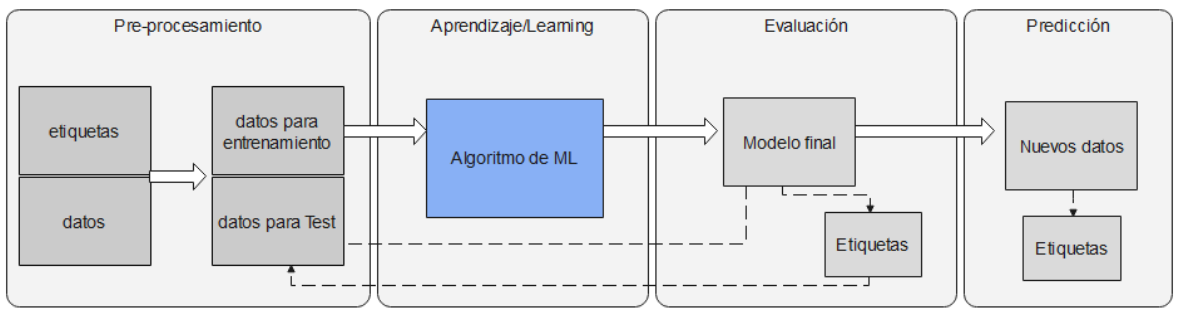
\includegraphics[width=1\textwidth]{tesis_1.png}
  	\caption{Diagrama de flujo de una aplicación de \textit{Machine Learning}.}
  	\label{fig:flowchartml.}
  	\end{center}
\end{figure}

Por tanto el Aprendizaje Automático es la generación de un modelo de predicción de salida a partir de grandes cantidades de datos de entrada, realizando un tratamiento de los mismos a través de diferentes etapas bien definidas, como se pueden apreciar en la Fig.~\ref{fig:flowchartml.}, las cuales iremos desarrollando en diferentes secciones.

Es importante destacar la independencia del aprendizaje automático al momento de tomar decisiones a partir de los datos proporcionados sin intervención externa, es decir que no hay una especificación de reglas que dictan cómo deben ser tomadas estas decisiones. A su vez, los modelos obtenidos a partir de los algoritmos de \textit{Machine Learning} deben tener la capacidad de predecir a partir de nuevos datos, nunca antes procesados por el modelo, a esto se lo conoce como \textbf{generalización}. 

\subsection{Preprocesamiento} \label{preprocessing}
Este punto es vital para cualquier proyecto que utiliza algoritmos de \textit{Machine Learning}, debido a que los datos incluidos en los conjuntos conocidos como \textit{datasets}, no suelen presentarse en condiciones para obtener el óptimo rendimiento de los algoritmos de aprendizaje. Estos datos suelen estar desbalanceados, haya faltantes o sean demasiado ruidosos, etc. 

Por lo tanto, una vez que se obtiene el \textit{dataset} de entrada, es primordial investigar, limpiar y transformar los datos con diversas técnicas, de forma que presentemos un conjunto de datos que esté en condiciones de ser entrenado y luego el modelo resultante, al momento de ser probado con datos desconocidos, tenga un desempeño óptimo.  

Para lograr este objetivo se aplican técnicas tales como normalización, reescalado, reducción de dimensionalidad, discretización, tratamiento de anomalías y \textit{outliers}. También de ser necesario se utilizan algoritmos de Aprendizaje no supervisado.

\subsection{Aprendizaje supervisado} \label{supervised}
El aprendizaje supervisado es el enfoque más utilizado y mejor entendido para el aprendizaje automático. Implica una entrada y salida para cada pieza de datos en su \textit{dataset}. 

Por ejemplo, una entrada podría ser una imagen y la salida podría ser la respuesta a ``?`es esto un gato?''. En el aprendizaje supervisado siempre hay una distinción entre el conjunto de entrenamiento o \textit{training} para el cual se nos proporciona la etiqueta (o \textit{label}), y el conjunto de test para el cual la etiqueta debe ser inferida. El algoritmo de aprendizaje debe ajustar el modelo predictivo al \textit{dataset} de entrenamiento y usamos el conjunto de test para evaluar la capacidad de generalización. El aprendizaje supervisado es ideal para tareas donde el modelo necesita predecir resultados. 

\textbf{Agregar validación, test, etc}

\textbf{features}

Estos problemas de predicción podrían involucrar el uso de estadísticas para predecir un valor (por ejemplo, $20 kg$, $\$1498$, $0.80 cm$) o categorizar datos basados en clasificaciones dadas (por ejemplo, ``gato'', ``verde'', ``feliz'') \cite{norman2019aprendizaje}.  El siguiente paso es profundizar en las dos categorías de aprendizaje supervisado que existen: clasificación y regresión.

\subsubsection{Clasificación}

En clasificación, la etiqueta es discreta, por ejemplo \texttt{Spam} y \texttt{No Spam}. En otras palabras, se proporciona una distinción clara entre las categorías. 

Es más, es importante indicar que estas categorías son nominales y no ordinales. Las variables nominales y ordinales son ambas subcategorías de las variables categóricas. Las variables ordinales tienen asociado un orden, por ejemplo, las tallas de las camisetas ``$XL > L > M > S$''. Por el contrario, las variables nominales no implican un orden, por ejemplo, no podemos asumir (en general) ``$naranja > azul > verde$'' \cite{GitHubpa25:online}.

\textbf{multilabel-etc}

Elegir entre dos categorías se denomina \textbf{clasificación binaria}, como lo es el ejemplo de \texttt{Spam} y \texttt{No Spam}, mientras que elegir entre más de dos categorías se denomina \textbf{clasificación multiclase}. 

Un ejemplo de clasificación multiclase podría ser clasificar un conjunto de imágenes de frutas, donde habrá manzanas, naranjas y peras. Es importante resaltar que si en el dataset de entrenamiento no aparece determinada categoría (por ejemplo bananas), nuestro modelo será incapaz de reconocer esa fruta.

\begin{figure}[H]
	\begin{center}				
	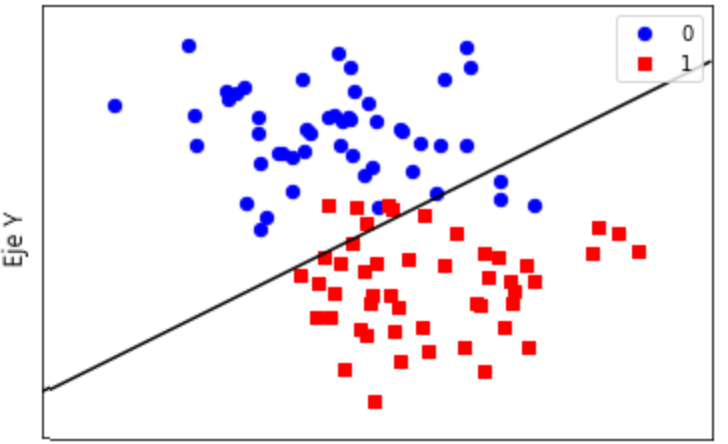
\includegraphics[width=0.5\textwidth]{tesis_2.png}
  	\caption{Ejemplo de clasificación binaria.}
  	\label{fig:binaryclassification.}
  	\end{center}
\end{figure}

Para poder apreciar el concepto de clasificación binaria, en la Fig.~\ref{fig:binaryclassification.}  \cite{GitHubpa25:online} se han graficado datos bidimensionales, es decir que cada dato tiene dos valores asociados de acuerdo a los ejes X e Y. El dataset cuenta con 100 muestras, las cuales están divididas en dos clases: ceros (círculos azules) y unos (cuadrados rojos). 

El modelo a utilizar para la predicción será uno de los más conocidos y simples de utilizar en clasificación, \textbf{regresión logística}. Éste es un modelo lineal, lo que significa que creará una frontera de decisión que es lineal en el espacio de entrada, en 2D esto quiere decir que generará una línea recta para separar los puntos azules de los rojos.

Como puede observarse, el modelo no es 100\% preciso ya que algunos puntos azules están en la categoría de los rojos y viceversa, por eso es que existen diversos modelos y debemos elegir según nuestro criterio cuál de ellos se adecúa mejor a nuestras necesidades.

Debido a la cantidad de diversos algoritmos que existen para clasificación es posible caracterizarlos en función de sus pros y contras como se observa en la Figura~\ref{fig:proconsclassification.}.

\begin{figure}[H]
	\begin{center}				
	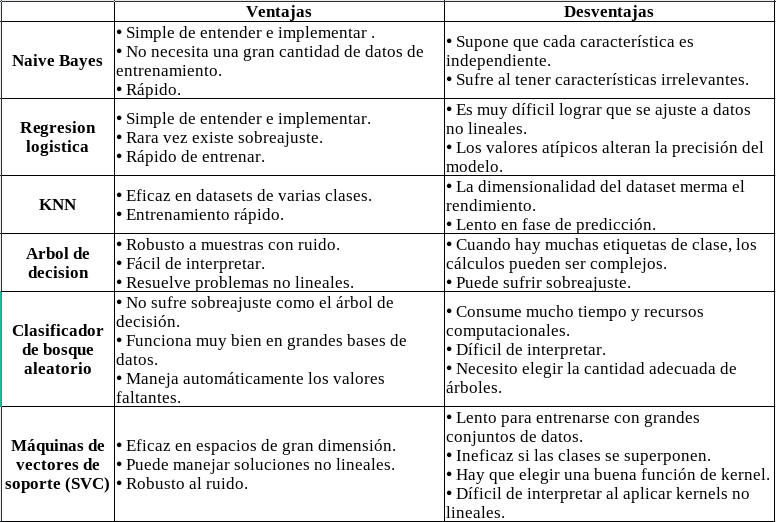
\includegraphics[width=1\textwidth]{tesis_6.png}
  	\caption{Ventajas y desventajas de los algoritmos de clasificación.}
  	\label{fig:proconsclassification.}
  	\end{center}
\end{figure}

\subsubsection{Regresión}

En regresión, la etiqueta es continua, es decir una salida real. Por ejemplo, en astronomía, la tarea de determinar si un objeto es una estrella, una galaxia o un cuásar es un problema de clasificación: la etiqueta viene de tres categorías distintas. Por otro lado, podríamos querer estimar la edad de un objeto basándonos en su imagen: esto sería regresión, porque la etiqueta (edad) es una cantidad continua \citep{GitHubpa25:online}.

En los problemas de regresión, tenemos como entradas las variables independientes o explicativas y las salidas o etiquetas son variables continuas. Por lo tanto, los modelos de regresión deben encontrar una relación (función lineal, polinomial, entre otras) que nos permitan predecir la salida.

\begin{figure}[]
	\begin{center}				
	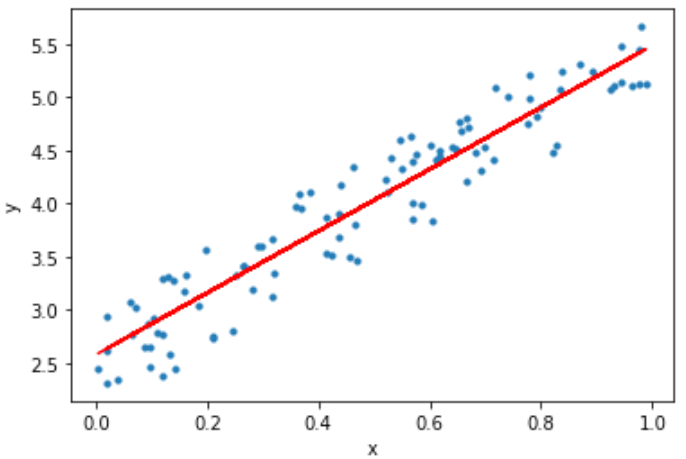
\includegraphics[width=0.5\textwidth]{tesis_9.png}
  	\caption{Ejemplo de regresión lineal.}
  	\label{fig:regressionlinear.}
  	\end{center}
\end{figure}

Para poder apreciar el concepto de regresión lineal, en la Fig.~\ref{fig:regressionlinear.} se tienen 100 muestras con sus respectivas etiquetas, entonces lo que hace el algoritmo de regresión lineal es ajustar una línea recta que minimice la distancia (en este caso distancia euclídea) entre los puntos de la muestra y dicha recta. Al obtener la recta, disponemos de los parámetros del modelo como son los coeficientes y la intersección, por ende estamos en condiciones de predecir la salida de nuevas muestras.

Así como pudimos listar las ventajas y desventajas con los distintos algoritmos de clasificación también es aplicable a los de regresión como vemos en la Fig.~\ref{fig:proconsregression.}.

\begin{figure}[H]
	\begin{center}				
	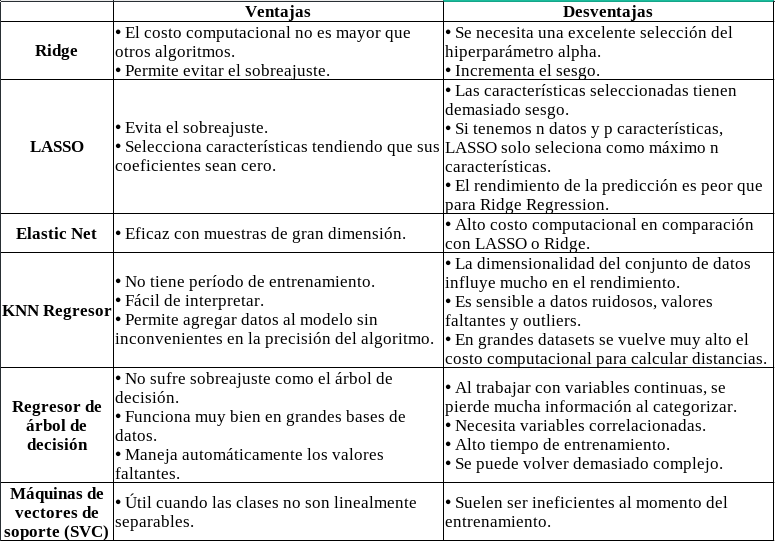
\includegraphics[width=1\textwidth]{tesis_10.png}
  	\caption{Ventajas y desventajas de los algoritmos de regresión.}
  	\label{fig:proconsregression.}
  	\end{center}
\end{figure}

\clearpage

\subsection{Aprendizaje no supervisado} \label{unsupervised}

A diferencia de lo que sucede en el aprendizaje supervisado (sección~\ref{supervised}), no disponemos de una salida deseada, tampoco se disponen datos etiquetados o con estructuras definidas. Por lo que el objetivo principal del Aprendizaje no Supervisado es generar esas etiquetas a partir de la información que se extrae de datos proporcionados en el \textit{dataset}, sin tener una referencia de salida.  

Un ejemplo de aprendizaje no supervisado podría ser si nos encontramos con un texto extenso y queremos obtener una especie de resumen, de los temas o tópicos relevantes, probablemente de antemano no se sabe cuales son o su cantidad, por lo tanto nos enfrentamos a la situación de no conocer cuales serian las salidas esperadas del modelo. 
Otros ejemplos clásicos pueden ser agrupar fotografías similares o separación de diferentes fuentes que originan un determinado sonido. 

Como se comentó anteriormente en la sección~\ref{preprocessing}, en la etapa de preprocesamiento, es muy útil aplicar las técnicas del aprendizaje no supervisado ya que se cuentan con grandes cantidades de datos en contextos no conocidos y lo más importante, sin etiquetar. Entonces suele ser una buena práctica dar un primer paso mediante algoritmos de aprendizaje no supervisado antes de pasar los datos a un proceso de aprendizaje supervisado. Como por ejemplo cuando se realizan transformaciones de datos mediante reescalado o estandarización. 

En las próximas subsecciones explicaremos brevemente cada una de las tareas que comprenden el Aprendizaje no Supervisado.

\subsubsection{Detección de anomalías}

Uno de los primeros pasos a realizar cuando se nos presenta un conjunto de datos, es proceder con la tarea llamada detección de anomalías (\textit{anomaly detection}, AD), o identificación de \textit{outliers} o datos fuera de rango. 

Un \textit{outlier} puede ser considerado como un dato atípico en un dataset. O bien “un \textit{outlier} es una observación en un dataset que parece ser inconsistente con el resto del conjunto”. Johnson 1992.

Tipos de entornos en los que se produce la detección de anomalías:
\begin{itemize}
	\item AD supervisada:
	\begin{itemize}
		\item Las etiquetas están disponibles, tanto para casos normales como para casos anómalos.
		\item En cierto modo, similar a minería de clases poco comunes o clasificación no balanceada.
	\end{itemize}
	\item AD semi-supervisada (detección de novedades, \textit{Novelty Detection})
	\begin{itemize}
		\item Durante el entrenamiento, solo tenemos datos normales.
		\item El algoritmo aprende únicamente usando los datos normales.
	\end{itemize}
	\item AD no supervisada (detección de \textit{outliers}, \textit{Outlier Detection})
	\begin{itemize}
		\item No hay etiquetas y el conjunto de entrenamiento tiene datos normales y datos anómalos.
		\item Asume que los datos anómalos son poco frecuentes.
		\item Algunos ejemplos típicos de detección de anomalías pueden ser, cuando se quiere detectar intrusos en tráfico de red o bien detectar acciones fraudulentas en transacciones con tarjetas de crédito.
	\end{itemize}
\end{itemize}

\begin{figure}[H]
	\begin{center}				
	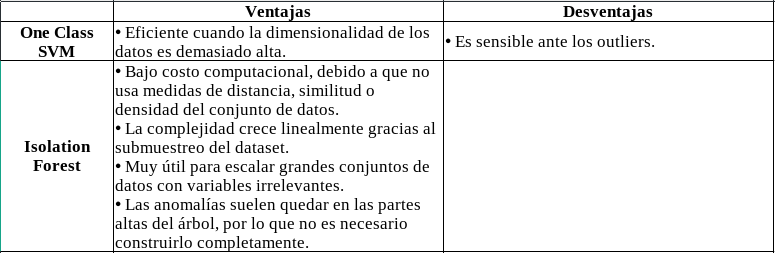
\includegraphics[width=1\textwidth]{tesis_11.png}
  	\caption{Ventajas y desventajas de los algoritmos de detección de anomalías.}
  	\label{fig:proconsanomaly.}
  	\end{center}
\end{figure}

\subsubsection{Reducción de dimensionalidad }

A menudo las muestras disponibles contienen una gran variedad de características, que pueden dar como resultado un sobreajuste del modelo utilizado, por lo tanto es necesario reducir la dimensionalidad de dichos datos pero manteniendo la información relevante. Al reducir la dimensionalidad no solo se evita el sobreajuste, sino que también se obtiene una mejor visualización de los datos y se reduce el costo computacional. 

Uno de los modelos más conocidos y que requieren menor costo computacional es Principal Component Analysis (PCA), pero si lo que estamos buscando es una mejor visualización de los datos y además las características no son lineales, sería recomendable usar T-SNE. 

\begin{figure}[H]
	\begin{center}				
	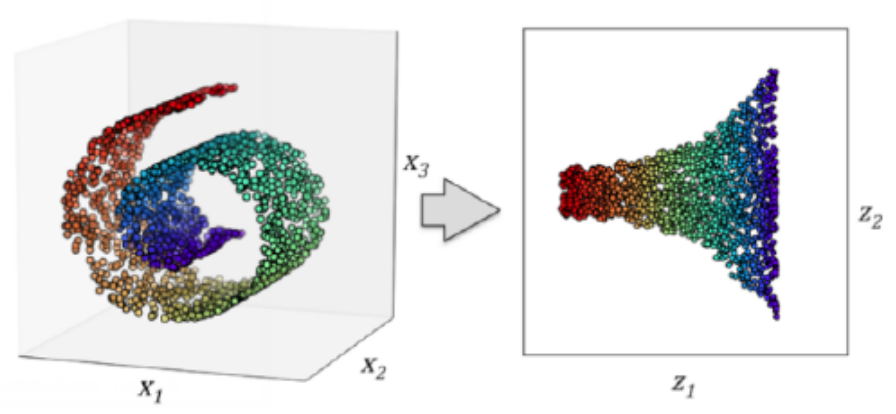
\includegraphics[width=0.7\textwidth]{tesis_12.png}
  	\caption{Reducción de dimensionalidad de 3D a 2D.}
  	\label{fig:reduxdimension.}
  	\end{center}
\end{figure}

En la Fig.~\ref{fig:reduxdimension.} \cite{trejoml} se muestra un ejemplo de cómo la reducción de dimensionalidad facilita la visualización de un dataset de alta dimensionalidad en una proyección de 1, 2 o 3 dimensiones.

Enumeramos en la Fig.~\ref{fig:proconsreduxdim.} las ventajas y desventajas de los algoritmos disponibles para esta tarea.

\begin{figure}[H]
	\begin{center}				
	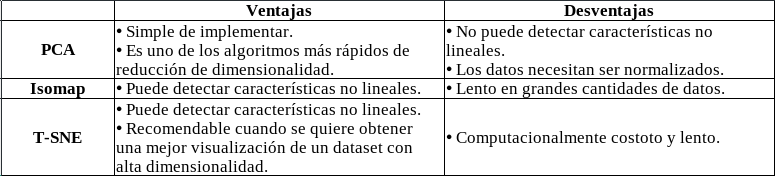
\includegraphics[width=1\textwidth]{tesis_15.png}
  	\caption{Pro y contras de algoritmos de reducción de dimensionalidad.}
  	\label{fig:proconsreduxdim.}
  	\end{center}
\end{figure}

\subsubsection{\textit{Clustering}}

El \textit{clustering} es una técnica que conceptualmente es simple de comprender, consiste agrupar objetos con características similares. Por lo tanto, obtenemos diferentes grupos llamados clústers, donde en cada uno de ellos están contenidos los datos que son más similares entre ellos que con los que pertenecen a otros clústers, obteniendo de esta forma una útil subdivisión del \textit{dataset}. Como no suele tenerse conocimiento sobre los datos, es decir no están etiquetados, esta técnica pertenece al Aprendizaje no Supervisado.

\clearpage

El algoritmo más simple de \textit{clustering} es K-means, el cual funciona para agrupar datos que se distribuyen en formas esféricas, si se usa la distancia euclídea. y a su vez hay que proporcionar la cantidad k de grupos en los cuales queremos distribuir el \textit{dataset}, por ello se debe tener un conocimiento previo de cuantos clúster se espera tener. 
Otras alternativas pueden ser, realizar \textit{clustering} jerárquico o \textit{clustering} basados en densidades.

En \textit{clustering} jerárquico, vemos como resultado un dendograma, es decir un diagrama de árbol. A partir de esto, se decide un umbral de profundidad, donde se corta el árbol y  de esta forma se obtiene un agrupamientos, por lo tanto a diferencia con K-means, no necesitamos tener información para poder decidir la cantidad de grupos. En la Fig.~\ref{fig:dendogram.} podemos observar como quedan evidenciados a través del dendograma los diferentes clusters.

\begin{figure}[H]
	\begin{center}				
	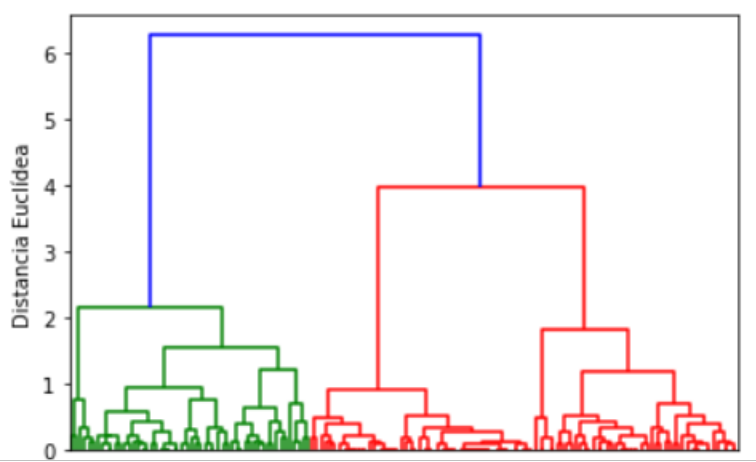
\includegraphics[width=0.6\textwidth]{tesis_16.png}
  	\caption{Dendograma generado por \textit{clustering} jerárquico.}
  	\label{fig:dendogram.}
  	\end{center}
\end{figure}

En cambio DBSCAN (\textit{Density-based Spatial Clustering of Applications with Noise}), divide el \textit{dataset} buscando las regiones densas de puntos, como podemos observar claramente en Fig.~\ref{fig:DBSCAN.}. Con esta técnica, tampoco especificamos el número de parámetros a priori, sino que se establecen hiperparámetros adicionales, como lo son la cantidad mínima de puntos y un radio $\epsilon$, para lograr un óptimo funcionamiento.

\begin{figure}[H]
	\begin{center}				
	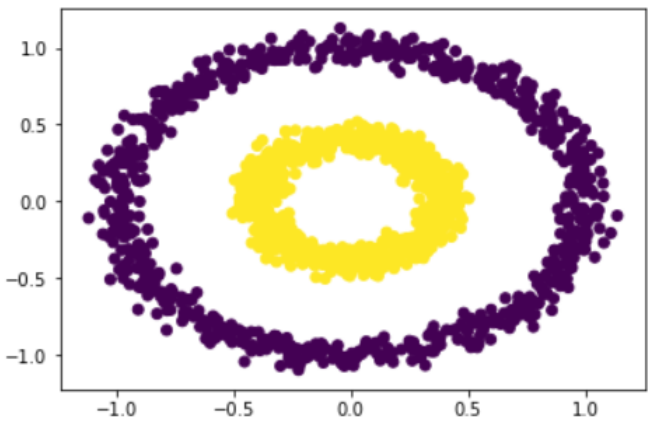
\includegraphics[width=0.6\textwidth]{tesis_17.png}
  	\caption{Clustering basado en densidades.}
  	\label{fig:DBSCAN.}
  	\end{center}
\end{figure}

Enumeramos en la Fig.~\ref{fig:proconsreduxdim.} las ventajas y desventajas de los algoritmos disponibles para esta tarea.

\begin{figure}[H]
	\begin{center}				
	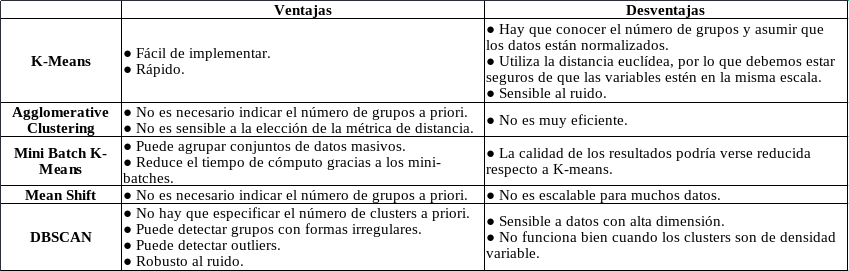
\includegraphics[width=1\textwidth]{tesis_34.png}
  	\caption{Pros y contras de los algoritmos de \textit{clustering}.}
  	\label{fig:proconsclustering.}
  	\end{center}
\end{figure}

\subsection{Selección de algoritmo en base al \textit{dataset}}
En la Fig.~\ref{fig:maindiagram.} obtenemos una vista general sobre que hacer con nuestros datos en función a nuestro objetivo.

\begin{figure}[H]
	\begin{center}				
	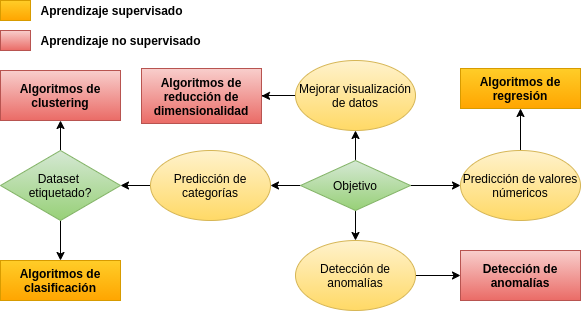
\includegraphics[width=1\textwidth]{maindiagram.png}
  	\caption{Diagrama general de algoritmos de aprendizaje supervisado y no supervisado.}
  	\label{fig:maindiagram.}
  	\end{center}
\end{figure}

\subsubsection{Algoritmos supervisados}

\begin{figure}[H]
	\begin{center}				
	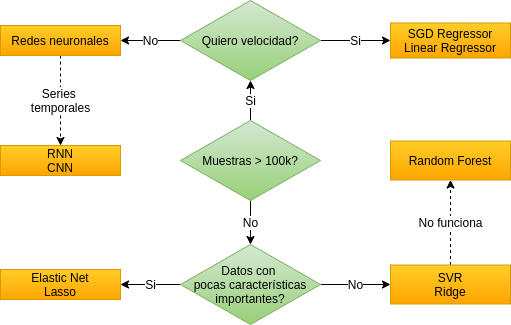
\includegraphics[width=0.9\textwidth]{regressiondiagram.png}
  	\caption{Diagrama general de los algoritmos de regresión.}
  	\label{fig:regressiondiagram.}
  	\end{center}
\end{figure}

\begin{figure}[H]
	\begin{center}				
	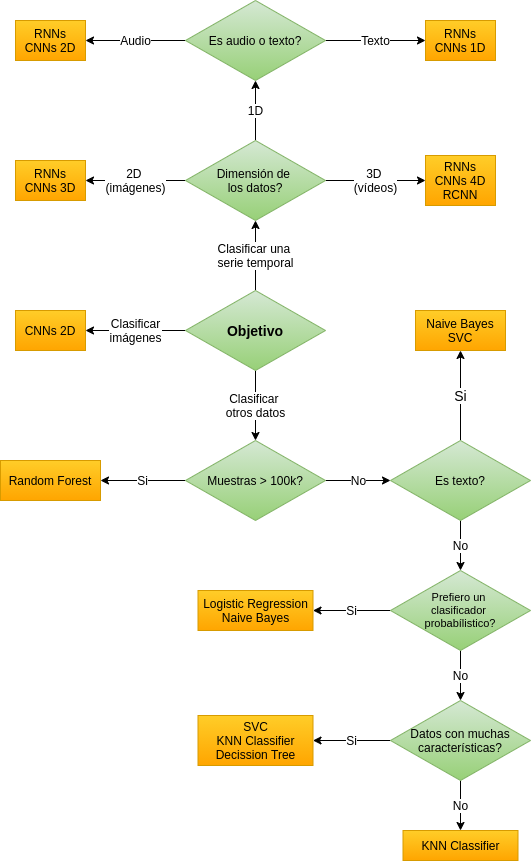
\includegraphics[width=0.9\textwidth]{classificationdiagram.png}
  	\caption{Diagrama general de los algoritmos de clasificación.}
  	\label{fig:classificationdiagram.}
  	\end{center}
\end{figure}

\subsubsection{Algoritmos no supervisados}

\begin{figure}[H]
	\begin{center}				
	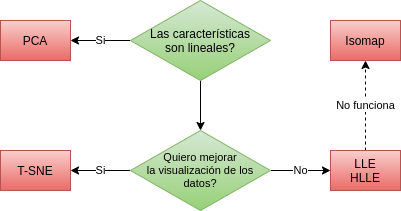
\includegraphics[width=0.8\textwidth]{dimreduxdiagram.png}
  	\caption{Diagrama general de los algoritmos de reducción de dimensión.}
  	\label{fig:dimreduxdiagram.}
  	\end{center}
\end{figure}

\begin{figure}[H]
	\begin{center}				
	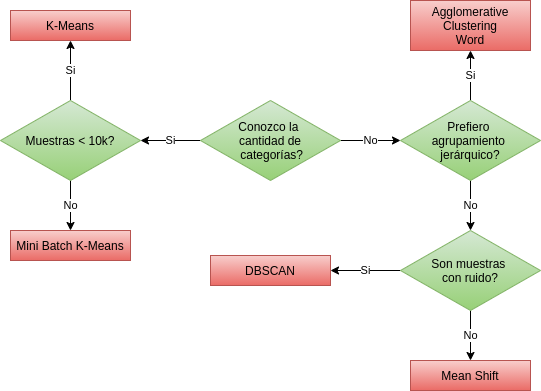
\includegraphics[width=0.9\textwidth]{clusteringdiagram.png}
  	\caption{Diagrama general de los algoritmos de \textit{clustering}.}
  	\label{fig:clusteringdiagram.}
  	\end{center}
\end{figure}

\begin{figure}[H]
	\begin{center}				
	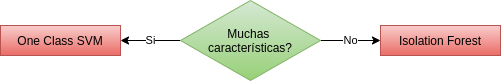
\includegraphics[width=0.9\textwidth]{anomalydiagram.png}
  	\caption{Diagrama general de los algoritmos de detección de anomalías.}
  	\label{fig:anomalydiagram.}
  	\end{center}
\end{figure}

\section{Redes neuronales}
La palabra neuronal es la forma adjetiva de "neurona", y red denota una estructura tipo grafo; por lo tanto, una \textit{Red Neuronal Artificial} es un sistema de computación que intenta imitar (o al menos, está inspirado en) las conexiones neuronales en nuestro sistema nervioso. Las redes neuronales artificiales también se denominan \textit{redes neuronales} o \textit{sistemas neuronales artificiales}. Es común abreviar la red neuronal artificial y referirse a ellas como "NN". \citep{rosebrock2017deep}

Para que un sistema se considere un NN, debe contener una estructura de grafo dirigida y etiquetada donde cada nodo del gráfico realice un cálculo simple. Según la teoría de grafos, sabemos que un gráfico dirigido consiste en un conjunto de nodos (es decir, vértices) y un conjunto de conexiones (es decir, bordes) que unen pares de nodos.

\begin{itemize}
\item Las entradas ingresan a la red. 
\item Cada conexión lleva una señal a través de las dos capas ocultas en la red. 
\item Una función final calcula la etiqueta de clase de salida.
\end{itemize}

\begin{figure}[H]
	\begin{center}				
	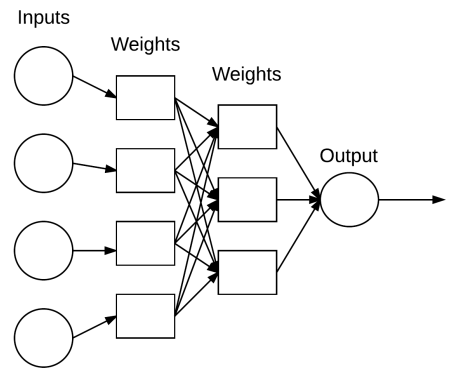
\includegraphics[width=0.6\textwidth]{018.png}
  	\caption{Arquitectura simple de red neuronal. \cite{matich}}
  	\label{fig:nn}
  	\end{center}
\end{figure}

Cada nodo realiza un cálculo simple. Cada conexión transporta una señal (es decir, la salida del cálculo) de un nodo a otro, marcada por un peso que indica el grado en que la señal se amplifica o disminuye. Algunas conexiones tienen grandes pesos positivos que amplifican la señal, lo que indica que la señal es muy importante al hacer una clasificación. Otros tienen pesos negativos, lo que disminuye la intensidad de la señal, lo que especifica que la salida del nodo es menos importante en la clasificación final. Llamamos a dicho sistema una Red Neuronal Artificial si consta de una estructura de grafo (como en la Figura \ref{fig:nn}) con pesos de conexión que se pueden modificar utilizando un algoritmo de aprendizaje.

\subsection{Relación con la biología}
Nuestros cerebros están compuestos por aproximadamente 10 mil millones de neuronas, cada una conectada a unas 10,000 otras neuronas. El cuerpo celular de la neurona se llama soma, donde las entradas (dendritas) y las salidas (axones) conectan el soma con otro (Figura \ref{fig:realneuron}).

\begin{figure}[H]
	\begin{center}				
	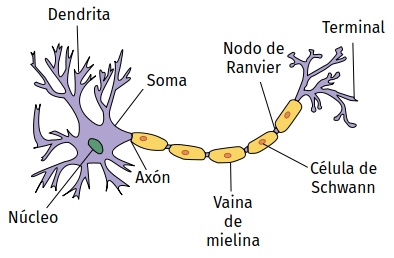
\includegraphics[width=0.6\textwidth]{019.png}
  	\caption{Estructura de una neurona biológica.}
  	\label{fig:realneuron}
  	\end{center}
\end{figure}


Cada neurona recibe entradas electroquímicas de otras neuronas en sus dendritas. Si estas entradas eléctricas son lo suficientemente potentes como para activar la neurona, entonces la neurona activada transmite la señal a lo largo de su axón, transmitiéndola a las dendritas de otras neuronas. Estas neuronas unidas también pueden activarse, continuando así el proceso de transmitir el mensaje.
La conclusión clave aquí es que el disparo de una neurona es una operación binaria: la neurona se dispara o no se dispara. No hay diferentes "grados" de disparo. En pocas palabras, una neurona solo se disparará si la señal total recibida en el soma excede un umbral dado.
Sin embargo, tenga en cuenta que los ANN simplemente se inspiran en lo que sabemos sobre el cerebro y cómo funciona. El objetivo del aprendizaje profundo no es imitar cómo funcionan nuestros cerebros, sino tomar las piezas que entendemos y permitirnos trazar paralelos similares en nuestro propio trabajo.

\subsection{Modelos artificiales}
Comencemos por ver un NN básico que realiza una suma ponderada simple de las entradas o \textit{inputs} en la Figura \ref{fig:simplenn}. Los valores $x_1$, $x_2$ y $x_3$ son las \textit{inputs} a nuestro NN y generalmente corresponden a una sola fila (es decir, punto de datos) de nuestra matriz de diseño. El valor constante 1 es nuestro sesgo o \textit{bias} que se supone incrustado en la matriz de diseño. Podemos pensar en estas \textit{inputs} como los vectores de características o \textit{features} de entrada a la NN.

\begin{figure}[H]
	\begin{center}				
	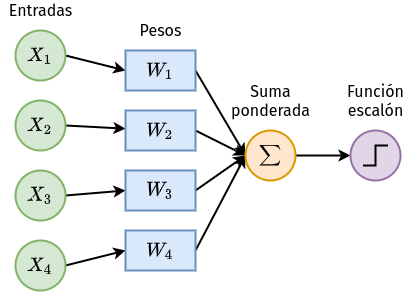
\includegraphics[width=0.6\textwidth]{020.png}
  	\caption{Simple NN.}
  	\label{fig:simplenn}
  	\end{center}
\end{figure}

Cada $x$ está conectada a una neurona a través de un vector de peso $W$ que consiste en $w_1, w_2, \ldots w_n$, lo que significa que para cada entrada $x$ también tenemos un peso asociado $w$.
Finalmente, el nodo de salida a la derecha toma la suma ponderada, aplica una función de activación $f$ (utilizada para determinar si la neurona se "dispara" o no) y genera un valor. Expresando la salida matemáticamente, normalmente encontrarás las siguientes tres formas:
\begin{itemize}
\item $f(w_1x_1 + w_2x_2 + \cdots + w_nx_n)$
\item $f(\sum_{i=1}^{n} w_ix_i)$	
\item O $f(net)$, donde $net = \sum_{i=1}^{n} w_ix_i$
\end{itemize}

\subsection{Funciones de activación}
La función de activación más simple es la "función de paso", utilizada por el algoritmo Perceptron.

$
f(net) =
\left\{
	\begin{array}{ll}
		1  	& \mbox{si } net > 0 \\
		0 	& \mbox{si } net \leq 0
	\end{array}
\right.
$

Esta es una función de umbral muy simple, sin embargo, aunque es fácil de usar e intuitiva, no es diferenciable, lo cual puede llevar a problemas cuando apliquemos el descenso por gradiente.
Por ello se presentan en la Figura \ref{fig:typesfactivation} diferentes tipos de funciones de activación con sus respectivos gráficos.

\begin{figure}[H]
	\begin{center}				
	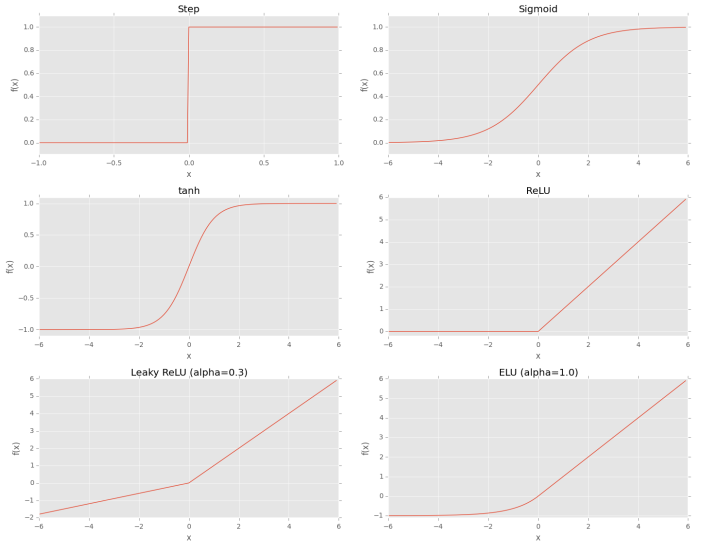
\includegraphics[width=1\textwidth]{021.png}
  	\caption{\textbf{Arriba-izquierda}: Función escalón. \textbf{Arriba-derecha}: Función sigmoidea. \textbf{Medio-izquierda}: Tangente hiperbólica. \textbf{Medio-derecha}: activación ReLU (función activación más usada en \textit{Deep Learning}).
 \textbf{Abajo-izquierda}: Leaky ReLU, variante de ReLU que permite valores negativos. \textbf{Abajo-derecha}:
ELU, otra variante de ReLU que obtiene mejor performance que Leaky ReLU.}
  	\label{fig:typesfactivation}
  	\end{center}
\end{figure}

Una de las funciones de activación más usadas en la historia de la literatura de NN es la función sigmoidea, que sigue la siguiente ecuación:

\begin{equation}
t=\sum_{i=1}^{n}w_ix_i \quad s(t)=\frac{1}{1+e^{-t}}
\end{equation}

La función sigmoidea es una mejor opción para el aprendizaje que la función de paso simple, ya que:
\begin{enumerate}
\item Es continua y diferenciable en todas partes.
\item Es simétrica alrededor del eje y.
\item Se acerca asintóticamente a sus valores de saturación.
\end{enumerate}
La principal ventaja aquí es que la suavidad de la función sigmoidea hace que sea más fácil diseñar algoritmos de aprendizaje. Sin embargo, hay dos grandes problemas con la función sigmoidea:
\begin{enumerate}
\item Las salidas del sigmoide no están centradas en cero.
\item Las neuronas saturadas esencialmente eliminan el gradiente, ya que el delta del gradiente será extremadamente pequeño.
\end{enumerate}

La tangente hiperbólica, o tanh (con una forma similar del sigmoide) también se usó fuertemente como una función de activación hasta fines de la década de 1990.
La ecuación para tanh sigue:
\begin{equation}
f(z) = tanh(z) = \frac{e^z - e^{-z}}{e^z + e^{-z}}
\end{equation}
La función tanh está centrada en cero, pero los gradientes aún se eliminan cuando las neuronas se saturan.
Ahora sabemos que hay mejores opciones para las funciones de activación que las funciones sigmoide y tanh. Específicamente, la Unidad Lineal Rectificada (ReLU), definida como:
\begin{equation}
f(x) = max(0, x)
\end{equation}
Las ReLU también se denominan "funciones de rampa" debido a cómo se ven cuando se trazan. La función es cero para entradas negativas pero luego aumenta linealmente para positivas valores. La función ReLU no es saturable y también es extremadamente  eficiente computacionalmente.
Empíricamente, la función de activación ReLU tiende a superar a las funciones sigmoide y tanh en casi todas las aplicaciones. Sin embargo, surge un problema cuando tenemos un valor de cero: no se puede tomar el gradiente.

\subsection{Arquitecturas de redes \textit{feedforward}}

Si bien hay muchas, muchas arquitecturas NN diferentes, la arquitectura más común es la red hacía adelante o \textit{feedforward}, como se presenta en la Figura \ref{fig:nnff}.

\begin{figure}[H]
	\begin{center}				
	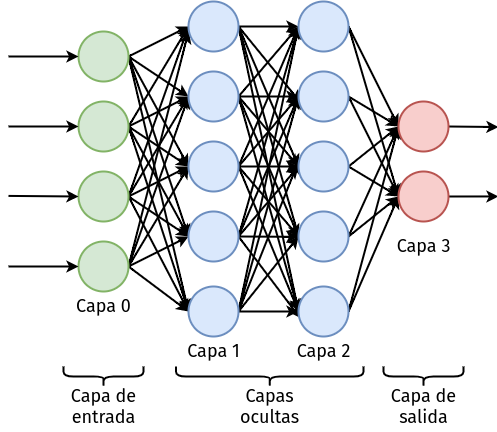
\includegraphics[width=0.65\textwidth]{022.png}
  	\caption{Un ejemplo de una red neuronal \textit{feedforward}.}
  	\label{fig:nnff}
  	\end{center}
\end{figure}

En este tipo de arquitectura, solo se permite una conexión entre los nodos de los nodos en la capa $i$ a los nodos en la capa $i + 1$ (de ahí el término \textit{feedforward}). No hay conexiones hacia atrás o entre capas permitidas. Cuando las redes de retroalimentación incluyen conexiones de retroalimentación (conexiones de salida que retroalimentan las entradas) se denominan redes neuronales recurrentes.

Para describir una red \textit{feedforward}, normalmente usamos una secuencia de enteros para depositar rápida y concisamente el número de nodos en cada capa. Por ejemplo, la red en la Figura 10.5 anterior es una red de alimentación directa 3-2-3-2:

\begin{itemize}
\item La capa 0 contiene 3 entradas, nuestros valores $x_i$. Estos podrían ser intensidades de píxeles sin procesar de una imagen o un vector de características extraído de la imagen.
\item Las capas 1 y 2 son capas ocultas que contienen 2 y 3 nodos, respectivamente.
\item La capa 3 es la capa de salida o la capa visible: allí es donde obtenemos la clasificación de salida general de nuestra red. La capa de salida generalmente tiene tantos nodos como etiquetas de clase; un nodo para cada salida potencial.
\end{itemize}

\subsection{Redes multicapa}
Las redes multicapas, \textit{i.e.} con varias capas de neuronas pueden ser modeladas matemáticamente como se muestra a continuación.
Supongamos $W$ como la matriz de pesos y el vector $b$ como el vector sesgo o \textit{bias}.
Consideremos:
\begin{equation}
z(x)=Wx+b=\sum_{i=1}^{n}w_ix_i+b
\end{equation}
Además cabe mencionar que la multiplicación punto a punto entre dos matrices de igual dimensión es lo que se conoce como el producto Hadamard.
\begin{equation}
\sigma(z)=\frac{1}{1+e^{-z}}
\end{equation}
Por último definimos la salida de nuestro modelo como:
\begin{equation}
\hat{y}=\sigma(\sum_{i=1}^{n}w_ix_i+b)
\end{equation}

\subsection{Función pérdida}

El objetivo del algoritmo de descenso de gradiente es minimizar la función de costo para que nuestro modelo neuronal pueda aprender.
Pero antes debemos definir que es la función costo o pérdida \cite{sgd}.
En el cálculo, los máximos (o mínimos) de cualquier función pueden ser descubiertos por:
\begin{enumerate}
\item Tomando la derivada de primer orden de la función e igualándola a 0. El punto encontrado de esta manera puede ser el punto de máximo o mínimo.
\item Sustituimos estos valores (el punto que acabamos de encontrar) en la derivada de segundo orden de la función y si el valor es positivo, \textit{i.e.}$>0$, entonces ese punto ($s$) representa el punto ($s$) de mínimos locales o máximos locales.
\end{enumerate}

Necesitamos cerrar la brecha entre la salida del modelo y la salida real. Cuanto menor sea la brecha, mejor será nuestro modelo en sus predicciones y más confianza mostrará al predecir.

La \textbf{función de pérdida o costo} esencialmente modela la diferencia entre la predicción de nuestro modelo y la salida real. Idealmente, si estos dos valores están muy separados, el valor de pérdida o el valor de error deberían ser mayores. Del mismo modo, si estos dos valores están más cerca, el valor del error debería ser bajo.
Una posible función de pérdida podría ser:
\begin{equation}
J(\Theta)=\hat{y}-y / y\in\{0,1\}
\end{equation}
Pero, en lugar de tomar esta función como nuestra función de pérdida, terminamos considerando la siguiente función:
\begin{equation}
J(\Theta)=\frac{\|\hat{y}-y\|^2}{2}
\end{equation}
Esta función se conoce como error al cuadrado . Simplemente tomamos la diferencia entre la salida real $y$ y la salida predicha $\hat{y}$ elevamos al cuadrado ese valor (de ahí el nombre) y lo dividimos entre 2.

Una de las principales razones para preferir el error al cuadrado en lugar del error absoluto es que el error al cuadrado es diferenciable en todas partes , mientras que el error absoluto no lo es (su derivada no está definida en 0).

Además, los beneficios de la cuadratura incluyen:
\begin{itemize}


\item La cuadratura siempre da un valor positivo , por lo que la suma no será cero.
\item Hablamos de suma aquí porque sumaremos los valores de pérdida o error para cada imagen en nuestro conjunto de datos de entrenamiento y luego haremos un promedio para encontrar la pérdida para todo el lote de ejemplos de entrenamiento.
\item La cuadratura enfatiza las diferencias más grandes, una característica que resulta ser buena y mala.

\end{itemize}

La función de error que usaremos aquí se conoce como el error cuadrático medio y la fórmula es la siguiente:

\begin{equation}
J(\Theta)=\frac{1}{2m} \sum_{i=1}^{m} (\hat{y_i}-y_i)^2
\label{funcperdida}
\end{equation}

Calculamos el error al cuadrado para cada \textit{feature} en nuestro \textit{dataset} y luego encontramos el promedio de estos valores y esto representa el error general del modelo en nuestro conjunto de entrenamiento.

Consideremos el ejemplo de una sola \textit{feature} con solo 2 características de antes. Dos características significan que tenemos 2 valores de peso correspondientes y un valor de sesgo. En total, tenemos 3 parámetros para nuestro modelo.

\begin{equation}
\hat{y} = w_1x_1 + w_2x_2 + b
\end{equation}

\begin{equation}
J(\Theta)=\frac{1}{2m} \sum_{i=1}^{m} (w_1x_1^{(i)}+w_2x_2^{(i)}+b-y^{(i)})^2
\end{equation}

Queremos encontrar valores para nuestros pesos y el sesgo que minimiza el valor de nuestra función de pérdida. Dado que esta es una ecuación de múltiples variables, eso significa que tendríamos que tratar con derivadas parciales de la función de pérdida correspondiente a cada una de nuestras variables $w_1$, $w_2$ y $b$.

\begin{equation}
\frac{\partial J}{\partial w_1} \frac{\partial J}{\partial w_2}
\frac{\partial J}{\partial b}
\end{equation}

Esto puede parecer lo suficientemente simple porque solo tenemos 3 variables diferentes.
Sin embargo tenemos tantos pesos como features \textit{i.e.} $w_n$ pesos.

Hacer una optimización multivariante con tantas variables es computacionalmente ineficiente y no es manejable. Por lo tanto, recurrimos a alternativas y aproximaciones.

\subsection{Descenso de gradiente}

Es la capacidad de aprendizaje que otorga el algoritmo de descenso de gradiente lo que hace que el aprendizaje automático y los modelos de aprendizaje profundo funcionen.

El objetivo de este algoritmo es minimizar el valor de nuestra función de pérdida y queremos hacer esto de manera eficiente.
Como se discutió anteriormente, la forma más rápida sería encontrar derivadas de segundo orden de la función de pérdida con respecto a los parámetros del modelo. Pero, eso es computacionalmente costoso.

La intuición básica detrás del descenso del gradiente puede ilustrarse mediante un escenario hipotético \citep{gdanalogy}: una persona está atrapada en las montañas y está tratando de bajar (es decir, tratando de encontrar los mínimos). Hay mucha niebla de tal manera que la visibilidad es extremadamente baja. Por lo tanto, el camino hacia abajo de la montaña no es visible, por lo que deben usar la información local para encontrar los mínimos.

Pueden usar el método de descenso en gradiente, que consiste en mirar la inclinación de la colina en su posición actual, luego proceder en la dirección con el descenso más empinado (es decir, cuesta abajo).
Si trataban de encontrar la cima de la montaña (es decir, los máximos), entonces avanzarían en la dirección con el ascenso más empinado (es decir, cuesta arriba). Usando este método, eventualmente encontrarían su camino.

Sin embargo, suponga también que la pendiente de la colina no es inmediatamente obvia con una simple observación, sino que requiere un instrumento sofisticado para medir, que la persona tiene en ese momento.

Se necesita bastante tiempo para medir la inclinación de la colina con el instrumento, por lo tanto, deben minimizar el uso del instrumento si quieren bajar la montaña antes del atardecer.
La dificultad es elegir la frecuencia con la que deben medir la inclinación de la colina para no desviarse.

En esta analogía:
\begin{itemize}

\item La persona representa nuestro \textbf{algoritmo de aprendizaje}, y
el camino que baja por la montaña representa la \textbf{secuencia de actualizaciones de parámetros} que nuestro modelo eventualmente explorará.
\item La inclinación de la colina representa la \textbf{pendiente de la superficie de error en ese punto}.
\item El instrumento utilizado para medir la inclinación es la \textbf{diferenciación} (la pendiente de la superficie de error se puede calcular tomando la derivada de la función de error al cuadrado en ese punto). Esta es la aproximación que hacemos cuando aplicamos el descenso de gradiente. Realmente no sabemos el punto mínimo, pero sí sabemos la dirección que nos llevará a los mínimos (locales o globales) y damos un paso en esa dirección.
\item La dirección en la que la persona elige viajar se alinea con el gradiente de la superficie de error en ese punto.
\item La cantidad de tiempo que viajan antes de tomar otra medida es la \textbf{velocidad de aprendizaje del algoritmo}. Esto es esencialmente lo importante que nuestro modelo (o la persona que va cuesta abajo) decide dar cada vez.

\end{itemize}

Entonces el descenso del gradiente mide el gradiente local de la función de pérdida (costo) para un conjunto dado de parámetros ($\Theta$) y da pasos en la dirección del gradiente descendente. Como ilustra la Figura \ref{fig:gd}, una vez que el gradiente es cero, hemos alcanzado un mínimo.

\begin{figure}[H]
	\begin{center}				
	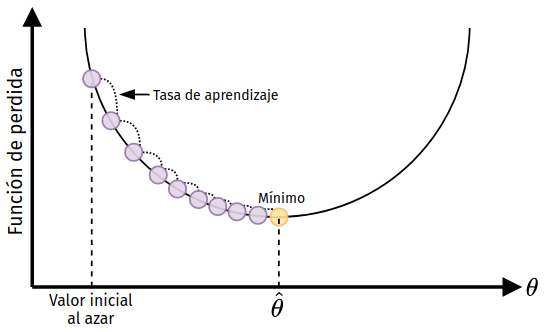
\includegraphics[width=0.65\textwidth]{023.png}
  	\caption{Representación gráfica del descenso de gradiente.}
  	\label{fig:gd}
  	\end{center}
\end{figure}

Como vemos en la Fig~\ref{fig:lr}.Es importante ajustar apropiadamente el valor de la tasa de aprendizaje \textit{(learning rate)}. Si es demasiado pequeña, entonces el algoritmo tomará muchas iteraciones (pasos) para encontrar el mínimo. Por otro lado, si es muy alta, es posible que supere el mínimo y termine más lejos que cuando comenzó.

\begin{figure}[H]
	\begin{center}				
	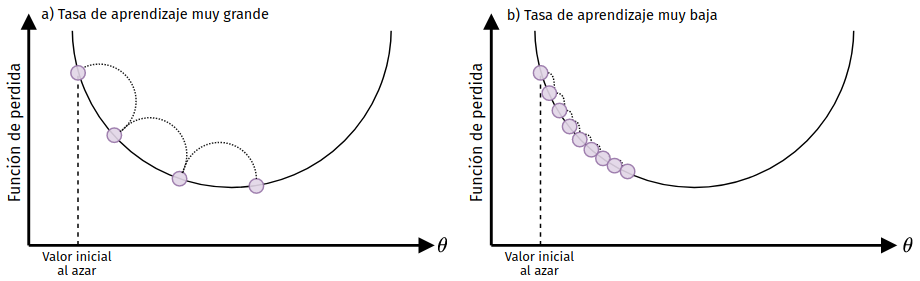
\includegraphics[width=1\textwidth]{tesis_37.png}
  	\caption{Ajuste de la tasa de aprendizaje.}
  	\label{fig:lr}
  	\end{center}
\end{figure}

Por tanto para actualizar la matriz de pesos y de sesgo serán utilizadas las siguientes ecuaciones.

\begin{equation}
W' = W - \alpha \frac{\partial J}{\partial W}
\end{equation}

\begin{equation}
b' = b - \alpha \frac{\partial J}{\partial b}
\end{equation}

El $\alpha$ representa la tasa de aprendizaje o  \textit{learning rate}.

\subsection{Backpropagation}

Ya sabemos cómo fluyen las activaciones en la dirección hacia adelante. Tomamos las \textit{features} de entrada, las transformamos linealmente, aplicamos la activación sigmoidea en el valor resultante y finalmente tenemos nuestra activación que luego usamos para hacer una predicción \citep{sgd}.

Lo que veremos en esta sección es el flujo de gradientes a lo largo de la línea roja en la Figura \ref{fig:back} mediante un proceso conocido como retropropagación o \textit{backpropagation}, que es esencialmente la regla de la cadena de cálculo aplicada a los gráficos computacionales.

\begin{figure}[H]
	\begin{center}				
	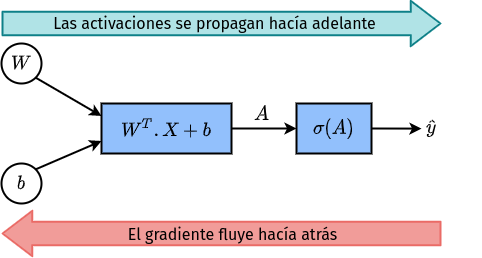
\includegraphics[width=0.65\textwidth]{024.png}
  	\caption{Las activaciones se propagan hacía adelante, pero los gradientes fluyen hacía atrás.}
  	\label{fig:back}
  	\end{center}
\end{figure}

Digamos que queríamos encontrar la derivada parcial de la variable $y$ con respecto a $x$ de la Figura \ref{fig:func}. No podemos descubrirlo directamente porque hay otras 3 variables involucradas en el gráfico computacional. Entonces, hacemos este proceso iterativamente yendo hacia atrás en el gráfico de cálculo.

Primero descubrimos la derivada parcial de la salida $y$ con respecto a la variable $C$. Luego usamos la regla de la cadena de cálculo y determinamos la derivada parcial con respecto a la variable $B$ y así sucesivamente hasta que obtengamos la derivada parcial que estamos buscando.

\begin{figure}[H]
	\begin{center}				
	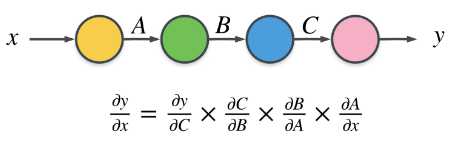
\includegraphics[width=0.65\textwidth]{025.png}
  	\caption{Representación de grafo simple.}
  	\label{fig:func}
  	\end{center}
\end{figure}

Utilizando la función pérdida definida en la ecuación \ref{funcperdida} y reescribiéndola en su forma vectorial.

\begin{equation}
J(\Theta)=\frac{1}{2} \|\hat{Y}-Y\|^2
\end{equation}

La derivada parcial de la función de pérdida con respecto a la activación de nuestro modelo es:

\begin{equation}
\frac{\partial J}{\partial \hat{Y}}
=\frac{1}{2} \frac{\partial J}{\partial \hat{Y}} \|\hat{Y}-Y\|^2 = \frac{1}{2} 2 \hat{Y} - Y \frac{\partial}{\partial \hat{Y}} (\hat{Y}-Y) = (\hat{Y}-Y) \frac{\partial}{\partial \hat{Y}} \|\hat{Y}-Y\| = (\hat{Y} - Y)
\label{dj/dy}
\end{equation}

Avancemos un paso hacia atrás y calculemos nuestra próxima derivada parcial. Esto nos llevará un paso más cerca de los gradientes reales que queremos calcular.

Este es el punto donde aplicamos la regla de la cadena que mencionamos antes. Entonces, para calcular la derivada parcial de la función de pérdida con respecto a la salida transformada lineal, es decir, la salida de nuestro modelo antes de aplicar la activación sigmoidea:

\begin{equation}
\frac{\partial J}{\partial D} = \frac{\partial J}{\partial \hat{Y}} \frac{\partial \hat{Y}}{\partial A}
\label{dJdD}
\end{equation}

La primera parte de esta ecuación es el valor que habíamos calculado en la ecuación \ref{dj/dy}. Lo esencial para calcular aquí es la derivada parcial de la predicción de nuestro modelo con respecto a la salida transformada linealmente.

Veamos la ecuación para la predicción de nuestro modelo, la función de activación sigmoidea.

\begin{equation}
\hat{Y} = \sigma(A) = \frac{1}{1+e^{-A}}
\end{equation}

Derivada de la salida final de nuestro modelo, \textit{i.e.} significa la derivada parcial de la función sigmoide con respecto a su entrada.

\begin{equation}
\frac{\partial}{\partial A} \sigma (A) = \frac{\partial}{\partial A} \frac{1}{1+e^{-A}} = \frac{\partial}{\partial A} (1+e^{-A})^{-1}
\end{equation}

\begin{equation}
 -1  (1+e^{-A})^{-2} \frac{\partial}{\partial A} (1+e^{-A}) = -1  (1+e^{-A})^{-2} (-e^{-A}) = \frac{e^{-A}}{(1+e^{-A})^2}
\end{equation}

Continuando, podemos simplificar aún más esta ecuación.

\begin{equation}
\sigma(A) = \frac{1}{1+e^{-A}}
\end{equation}

\begin{equation}
e^{-A} = \frac{1}{\sigma (A)} - 1 = \frac{1-\sigma (A)}{\sigma(A)}
\end{equation}

Substituyendo este valor en la ecuación \ref{dJdD} obtenemos:

\begin{equation}
\frac{\partial J}{\partial A} = \frac{\partial J}{\partial \hat{Y}} \frac{e^{-A}}{(1+e^{-A})^2}
\end{equation}

\begin{equation}
\frac{\partial J}{\partial A} = \frac{\partial J} {\partial \hat{Y} } \frac{1-\sigma(A)}{\sigma(A)} \sigma (A) \sigma (A)
\end{equation}

\begin{equation}
\frac{\partial J}{\partial A} = \frac{\partial J} {\partial \hat{Y}} \sigma(A) (1-\sigma(A))
\end{equation}

Necesitamos la derivada parcial de la función de pérdida correspondiente a cada uno de los pesos. Pero como estamos recurriendo a la vectorización, podemos encontrarlo todo de una vez. Es por eso que hemos estado usando la notación mayúscula $W$ en vez de $w_1, w_2, \ldots, w_n$.

\begin{equation}
\frac{\partial J}{\partial W} = \frac{\partial J}{\partial A} \frac{\partial A}{\partial W}
\label{dJ/dW}
\end{equation}

\begin{equation}
\frac{\partial J}{\partial b} = \frac{\partial J}{\partial A} \frac{\partial A}{\partial b}
\label{dJ/db}
\end{equation}

La derivación de los pesos queda partiendo de la ecuación \ref{dJ/dW}:

\begin{equation}
\frac{\partial J}{\partial W} = \frac{\partial J}{\partial A} \frac{\partial}{\partial W}(W^T X + b) = \frac{\partial J}{\partial A} X
\end{equation}

Y de la ecuación \ref{dJ/db}:

\begin{equation}
\frac{\partial J}{\partial b} = \frac{\partial J}{\partial A} \frac{\partial}{\partial b}((W^T X + b) = \frac{\partial J}{\partial A} 1 = \frac{\partial J}{\partial A}
\end{equation}

Se demostró desde un punto de vista matemático el concepto de \textit{backpropagation} como se realiza la actualización de los pesos y sesgos utilizando el descenso por gradiente.

\subsection{Descenso de gradiente estocástico (SGD)}
Sin embargo el descenso de gradiente puede ser excepcionalmente lento en datasets muy grandes debido a que en cada iteración requiere calcular una predicción por cada punto de entrenamiento en nuestros datos de entrenamientos antes que actualizaciones nuestra matriz de pesos.

En cambio lo que se utiliza es una variante de éste, el descenso de gradiente estocástico o \textit{Stochastic Gradient Descent (SGD)}.
El SGD es una simple modificación del algoritmo de descenso de gradiente estándar que computa el gradiente y actualiza la matriz de pesos $W$ en pequeños lotes o \textit{batches} de datos de entrenamiento, en vez del \textit{dataset} entero. Mientras esta modificación nos lleva a actualizaciones más " ruidosas", también nos permite tomar más pasos a lo largo del gradiente, llevando en ultima instancia a una convergencia más rápida y sin afectar negativamente a la pérdida y precisión del modelo.

En lugar de calcular nuestro gradiente en todo el conjunto de datos, en su lugar muestreamos nuestros datos, produciendo un lote. Evaluamos el gradiente en el lote y actualizamos nuestra matriz de peso W. Desde una perspectiva de implementación, también tratamos de aleatorizar nuestras muestras de entrenamiento antes de aplicar SGD ya que el algoritmo es sensible a los lotes.

En una implementación "purista" de SGD, el tamaño de su mini lote sería 1, lo que implica que muestrearíamos aleatoriamente un punto de datos del conjunto de entrenamiento, calcularíamos el gradiente
y actualizamos nuestros parámetros.

Sin embargo, a menudo utilizamos mini lotes que son mayores a 1. Los tamaños de lote típicos incluyen 32, 64, 128 y 256.

A continuación enumeramos las justificaciones a esta decisión.

\begin{enumerate}
\item Ayudan a reducir la variación en la actualización de parámetros, lo que conduce a una convergencia más estable. 
\item Las potencias de dos a menudo son deseables para los tamaños de lote, ya que permiten que las bibliotecas de optimización de álgebra lineal interna sean más eficientes.
\end{enumerate}
En general, el tamaño del mini lote no es un hiperparámetro por el que debería preocuparse demasiado. Si está usando una GPU para entrenar su red neuronal, usted determina cuántos ejemplos de entrenamiento encajarán en su GPU y luego usa la potencia más cercana de dos, ya que el tamaño del lote se ajustará en la GPU. Para el entrenamiento de CPU, normalmente utiliza uno de los tamaños de lote enumerados anteriormente para asegurarse de cosechar los beneficios de las bibliotecas de optimización de álgebra lineal.

\subsection{Sobreajuste y bajo-ajuste}
El sobreajuste o \textit{overfitting} y la falta de ajuste o \textit{underfitting} \cite{quora} es muy importante para saber si el modelo predictivo está generalizando bien los datos o no. Un buen modelo debe poder generalizar bien los datos.

\begin{figure}[H]
	\begin{center}				
	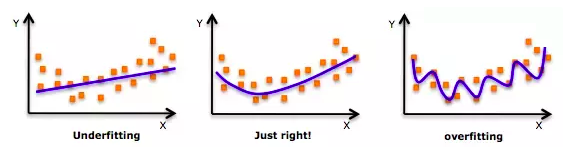
\includegraphics[width=0.8\textwidth]{026.png}
  	\caption{Distintas representaciones del ajuste en un mismo modelo.}
  	\label{fig:fitting}
  	\end{center}
\end{figure}

En la Figura \ref{fig:fitting} \textbf{Izquierda} el modelo está sobreajustado, \textit{i.e.} cuando funciona bien en el ejemplo de entrenamiento pero no funciona bien en datos no vistos. A menudo es el resultado de un modelo excesivamente complejo y ocurre porque el modelo está memorizando la relación entre el ejemplo de entrada (a menudo llamado $X$) y la variable objetivo (a menudo llamada $y$) o, por lo tanto, no puede generalizar bien los datos. El modelo de sobreajuste predice el objetivo en el conjunto de datos de entrenamiento con mucha precisión.

En cambio en la Figura \ref{fig:fitting} \textbf{Derecha} se dice que el modelo predictivo tiene bajo-ajuste, si funciona mal en los datos de entrenamiento. Esto sucede porque el modelo no puede capturar la relación entre el ejemplo de entrada y la variable objetivo. Podría deberse a que el modelo es demasiado simple, es decir, las características de entrada no son lo suficientemente expresivas como para describir bien la variable objetivo. El modelo con bajo-ajuste no predice los objetivos en los conjuntos de datos de entrenamiento con mucha precisión.

Un buen modelo debe ser como el de la Figura \ref{fig:fitting} \textbf{Medio} que posee una buena precisión en su conjunto de datos de entrenamiento pero a su vez también tiene una buena \textit{performance} con datos que no haya visto.

\subsection{Regularización}
Para disminuir los efectos del sobreajuste se utiliza la \textbf{regularización} que después de la tasa de aprendizaje, es el parámetro más importante de su modelo que puede ajustar.

Existen varios tipos de técnicas de regularización, como la regularización L1, la regularización L2 (comúnmente llamada “pérdida de peso”) y Elastic Net, que se utilizan al actualizar la función de pérdida en sí, agregando un parámetro adicional para restringir la capacidad de el modelo.

La regularización nos ayuda a controlar la capacidad de nuestro modelo, asegurando que nuestros modelos sean mejores para hacer clasificaciones (correctas) en los puntos de datos en los que no fueron entrenados, lo que llamamos la capacidad de generalizar. Si no aplicamos la regularización, nuestros clasificadores pueden volverse demasiado complejos y ajustarse fácilmente a nuestros datos de entrenamiento, en cuyo caso perdemos la capacidad de generalizar a nuestros datos de prueba.

\subsection{Los cuatro ingredientes de una red neuronal}
Hay cuatro ingredientes principales \citep{rosebrock2017deep} que necesita para armar su propia red neuronal y algoritmo de aprendizaje profundo: un conjunto de datos, un modelo/arquitectura, una función de pérdida y una optimización.
\subsubsection{Conjunto de datos}
También llamado \textit{dataset}, es el primer ingrediente en el entrenamiento de una red neuronal: los datos en sí mismos junto con el problema que estamos tratando de resolver definen nuestros objetivos finales.

La combinación de su conjunto de datos y el problema que está tratando de resolver influye en su elección en la función de pérdida, la arquitectura de red y el método de optimización utilizado para entrenar el modelo. Por lo general, tenemos pocas opciones en nuestro conjunto de datos (a menos que esté trabajando en un proyecto de pasatiempo): se nos da un conjunto de datos con cierta expectativa sobre cuáles deberían ser los resultados de nuestro proyecto. Depende de nosotros entrenar un modelo de aprendizaje automático en el conjunto de datos para que funcione bien en la tarea dada.

\subsubsection{Función de pérdida}
Dado nuestro conjunto de datos y objetivo objetivo, necesitamos definir una función de pérdida que se alinee con el problema que estamos tratando de resolver.

\subsubsection{Modelo/Arquitectura}
La arquitectura de su red puede considerarse la primera "elección" real que tiene que hacer como ingrediente. Es probable que su conjunto de datos sea elegido para usted (o al menos ha decidido que desea trabajar con un conjunto de datos determinado). Y si está realizando una clasificación, probablemente utilizará la entropía cruzada como su función de pérdida.
Sin embargo, su arquitectura de red puede variar dramáticamente, especialmente cuando con qué método de optimización elige entrenar su red.

\subsubsection{Método de optimización}
El ingrediente final es definir un método de optimización. El SGD se usa con bastante frecuencia.
SGD sigue siendo el caballo de batalla del aprendizaje profundo: la mayoría de las redes neuronales se entrenan a través de SGD, aunque existen otros métodos de optimización como Adam.
Luego debe establecer una tasa de aprendizaje adecuada, la fuerza de regularización y el número total de épocas para las que se debe entrenar la red.

\section{Redes neuronales convolucionales}
Las redes neuronales convolucionales \citep{rosebrock2017deep} (\textit{CNNs} en Inglés) son principalmente útiles si en la entrada los datos presentados son imágenes, permite el desarrollo de modelos supervisados y no supervisados.

Podemos definir una \textit{CNN} como una red neuronal que cambia una capa totalmente conectada (\textit{fully-connected}) por una convolucional para al menos una de las capas de la red.

Cada capa en una \textit{CNN} aplica un conjunto de filtros, usualmente cientos o miles de ellos y combinan los resultados, alimentando la entrada de la siguiente capa de la red. Durante el entrenamiento, una \textit{CNN} automáticamente aprende los valores para esos filtros.

En el contexto de la clasificación de imágenes, una \textit{CNN} puede aprender a:
\begin{itemize}
	\item Detectar bordes a partir de datos de píxeles sin procesar en la primera capa.
	\item Usar esos bordes para detectar formas (\textit{i.e. blobs}) en la segunda capa.
	\item Usar esas formas para detectar características de alto nivel tales como estructuras faciales, partes de un auto, etc. en las capas de más alto nivel.
\end{itemize}

La última capa en una \textit{CNN} usa esas características de alto nivel para realizar predicciones considerando los contenidos de una imagen.

Las \textit{CNNs} nos dan dos beneficios claves con respecto al reconocimiento de imágenes:
\begin{itemize}
	\item \textbf{invariancia local}: nos permite clasificar una imagen que contiene un objeto particular sin importar donde aparece éste en la imagen.
	\item \textbf{composicionalidad}: cada filtro compone un parche local de características de nivel inferior en una representación de nivel superior, similar a cómo podemos componer un conjunto de funciones matemáticas que se basan en la salida de funciones anteriores. Esta composición permite que nuestra red aprenda características más ricas de forma más profunda.

\end{itemize}

Las convoluciones bi-dimensionales (2D) son usadas para tratar las imágenes, mientras que las convoluciones unidimensionales (1D) nos permiten analizar entradas secuenciales, obteniendo la información con dependencias temporales. Entonces al combinar estas dos técnicas, se puede apreciar cómo evolucionan en el tiempo las imágenes capturadas y así hacer predicciones a futuro.

\subsection{Convolución 1D}
Si $f$ y $g$ son funciones discretas \citep{keller}, entonces $f * g$ es la convolución de $f$ y $g$ y está definida como:

$$(f*g)(x)=\sum_{u=-\infty}^{\infty} f(u)g(x-u)$$

Intuitivamente, la convolución de dos funciones representa la cantidad de superposición entre estas. La función $g$ es la entrada y $f$ el \textit{kernel} o núcleo de la convolución.

Sin embargo en los algoritmos de \textit{machine learning} lo que manejamos usualmente son vectores o arreglos de tal forma que nos resultará más provechoso analizar la convolución entre ellos.

Si la función $f$ varía sobre un conjunto finito de valores $a = a_1, a_2, \dots, a_n$ entonces puede ser representado como el vector 
$\begin{bmatrix} a_1 & a_2 & \cdots & a_n \end{bmatrix}$.

Si las funciones $f$ y $g$ son representadas como vectores $a = \begin{bmatrix} a_1 & a_2 & \cdots & a_m \end{bmatrix}$ y $b = \begin{bmatrix} b_1 & b_2 & \cdots & b_n \end{bmatrix}$, entonces $f*g$ es un vector $c = \begin{bmatrix} c_1 & c_2 & \cdots & c_{m+n-1} \end{bmatrix}$ definido de la siguiente forma:

$$ c = \sum_{u} a_u b_{x-u+1}$$

donde $u$ abarca todos los subíndices legales para $a_u$ y $b_{x-u+1}$, específicamente $u=max(1, x-n+1)\dots min(x,m).$

Lo que puede parecer complicado en la teoría no lo es en la práctica, observemos la Fig.~\ref{fig:conv1dk1} \citep{Cogneethi2019Aug}. El vector \textit{input} también se denomina vector de características y el vector \textit{output} mapa de características.

Lo que sucede es que si el \textit{kernel} tiene un único valor sólo es necesario multiplicarlo por cada valor del vector \textit{input} y guardarlo en el índice correspondiente del vector \textit{output}.

\begin{figure}[H]
	\begin{center}				
	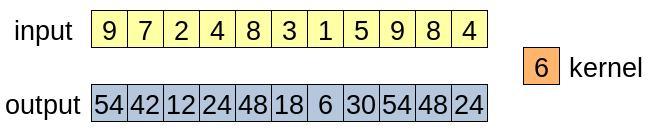
\includegraphics[width=0.65\textwidth]{tesis_24.png}
  	\caption{Vectores de convolución unidimensional con kernel simple.}
  	\label{fig:conv1dk1}
  	\end{center}
\end{figure}

En cambio si tenemos un \textit{kernel} de dimensiones $2 \times 1$ como la Fig.\ref{fig:conv1dk2} para obtener el valor de salida $i$ debemos usar los valores de entrada $i$ y su vecino $i+1$.

Para obtener el primer valor del vector de salida se realizó la operación \texttt{o[0] = i[0]k[0] + i[1]k[1] = 69}. De esta forma iteramos a lo largo de todo el vector de entrada hasta obtener todos los valores de salida. Podemos notar que el tamaño del vector de salida es menor ahora, a medida que aumentamos el tamaño del kernel disminuye el del vector de salida.

\begin{figure}[H]
	\begin{center}				
	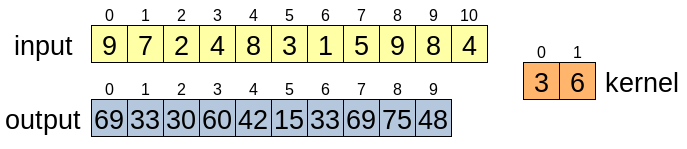
\includegraphics[width=0.7\textwidth]{tesis_25.png}
  	\caption{Vectores de convolución unidimensional con kernel doble.}
  	\label{fig:conv1dk2}
  	\end{center}
\end{figure}

Con objeto de dejar totalmente en claro el algoritmo observemos la Fig.~\ref{fig:conv1dk3}. Para obtener el valor del índice 4 del vector de salida operamos \texttt{o[4] = i[3]k[0]+i[4]k[1]+i[5]k[2] = 23}.

\begin{figure}[H]
	\begin{center}				
	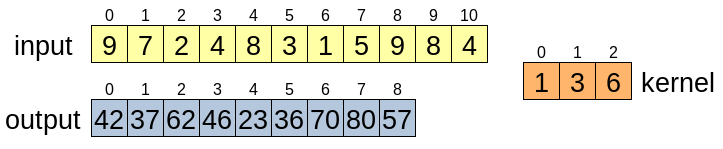
\includegraphics[width=0.75\textwidth]{tesis_26.png}
  	\caption{Vectores de convolución unidimensional con kernel triple.}
  	\label{fig:conv1dk3}
  	\end{center}
\end{figure}

Para finalizar se hará una pequeña mención al tamaño del vector de salida, que viene determinado por la siguiente formula \citep{SOOutputConv}:

$$ output_{size} = \frac{W-F+2P}{S+1}$$

donde $W = input_{size}$, $F=kernel_{size}$, $P$=\textit{padding} y $S$=\textit{stride}.

\subsection{Convolución 2D}

A su vez podemos extender esto a convoluciones para funciones de dos variables.

Si $f$ y $g$ son funciones discretas de dos variables, entonces $f*g$ es la convolución de $f$ y $g$ y se define:

$$
(f*g)(x,y) = \sum_{u=-\infty}^{+\infty} \sum_{v=-\infty}^{+\infty} f(u,v)g(x-u,y-v)
$$

Podemos considerar funciones de dos variables como matrices con $A_{xy} = f(x,y)$ y obtener una definición matricial de la convolución.

Si las funciones $f$ y $g$ son representadas como las matrices $A$ y $B$ con dimensiones de $n \times m$ y $k \times i$ respectivamente, entonces $f*g$ es una matriz $C$ de dimensiones $(n+k-1) \times (m+i-1)$ definida:

$$
c_{xy} = \sum_{u} \sum_{v} a_{uv} b_{x-u+1,y-v+1}
$$

donde $u$ y $v$ abarcan todos los subíndices posibles para $a_{uv}$ y $b_{x-u+1,y-v+1}$.

Así como notamos que el algoritmo para la convolución 1D no era tan complejo como su definición formal, lo mismo sucede para la convolución 2D pero extrapolando el mecanismo a una dimensión más.

En la Fig.~\ref{fig:conv2d} \citep{andrianaivo2019architecture} analizamos el procedimiento. Se debe centrar el kernel $K$ sobre el primer valor a calcular, para luego realizar las respectivas multiplicaciones y luego guardarlas en la matriz de salida $O$, de esta manera iremos iterando de derecha a izquierda y de arriba hacia abajo toda la matriz $I$.

\begin{figure}[H]
	\begin{center}				
	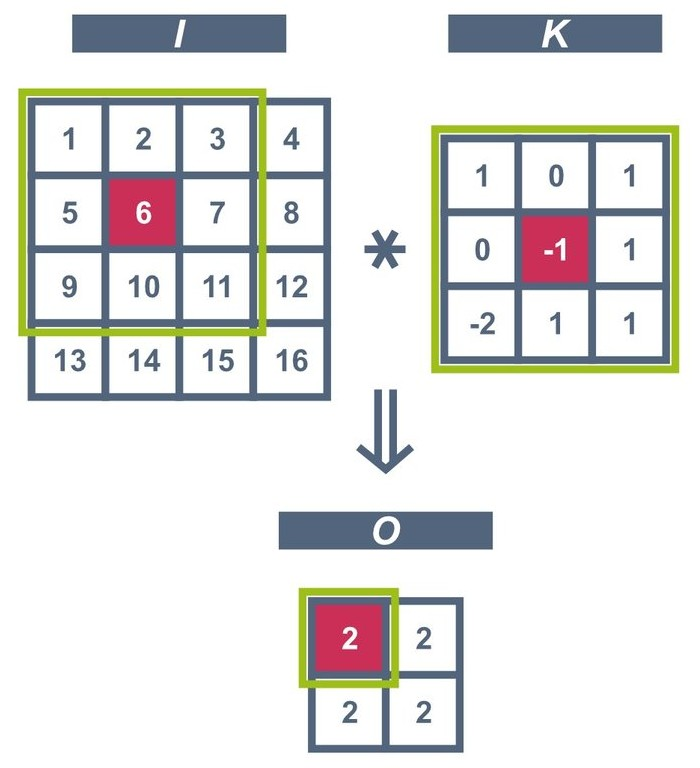
\includegraphics[width=0.4\textwidth]{convolution2d.jpg}
  	\caption{Vectores de convolución bidimensional con kernel $3 \times 3$.}
  	\label{fig:conv2d}
  	\end{center}
\end{figure}

Consideremos la Fig.~\ref{fig:conv2dimg} \citep{Saha2020Oct}, tenemos una imagen RGB que ha sido separada por sus tres canales de color: rojo, verde y azul. Hay varios espacios de color en los que existen las imágenes: escala de grises, RGB, HSV, CMYK, etc.

\begin{figure}[H]
	\begin{center}				
	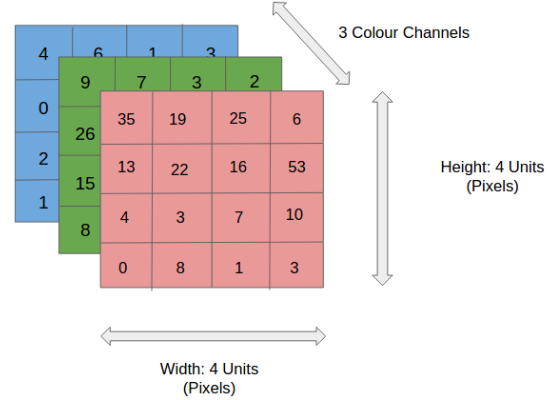
\includegraphics[width=0.7\textwidth]{imgrgb.png}
  	\caption{Imagen RGB $4 \times 4 \times 3$.}
  	\label{fig:conv2dimg}
  	\end{center}
\end{figure}

Si consideramos la totalidad de la imagen como un prisma donde la profundidad corresponde a cada canal de color, podemos ver en la Figura~\ref{fig:kernelmove} el movimiento que realiza el kernel (con forma de cubo) a través del volumen del prisma.

\begin{figure}[H]
	\begin{center}				
	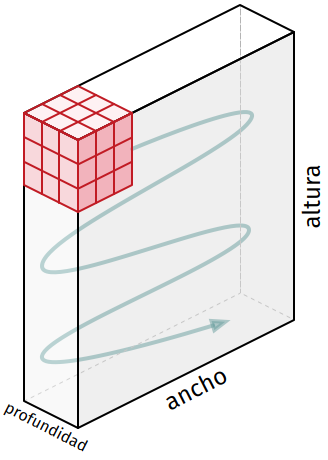
\includegraphics[width=0.3\textwidth]{kernelmove.png}
  	\caption{Movimiento del \textit{kernel}.}
  	\label{fig:kernelmove}
  	\end{center}
\end{figure}

\subsubsection{\textit{Padding}}

Un problema a abordar al aplicar la convolución es que tendemos a perder píxeles en el perímetro de nuestra imagen (o vector). Dado que normalmente usamos núcleos pequeños, para cualquier convolución dada, es posible que solo perdamos unos pocos píxeles, pero esto puede sumarse a medida que aplicamos muchas capas convolucionales sucesivas. Una solución sencilla a este problema es agregar píxeles adicionales de relleno (\textit{padding}) alrededor del límite de nuestra imagen de entrada, aumentando así el tamaño efectivo de la imagen. Normalmente, establecemos los valores de los píxeles adicionales en cero. \citep{padding}

En la figura~\ref{fig:padding}, rellenamos una entrada de $3 \times 3$, aumentando su tamaño a $5 \times 5$. La salida correspondiente aumenta entonces a una matriz de $4 \times 4$.

\begin{figure}[H]
	\begin{center}				
	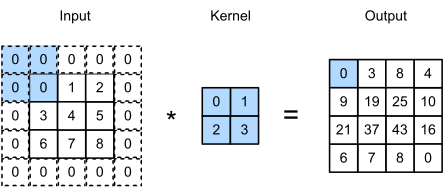
\includegraphics[width=0.6\textwidth]{conv-pad.png}
  	\caption{Relleno o \textit{padding}.}
  	\label{fig:padding}
  	\end{center}
\end{figure}

\subsubsection{\textit{Stride}}

Al realizar la convolución, comenzamos con la ventana en la esquina superior izquierda del tensor de entrada y luego la deslizamos sobre todas las ubicaciones, tanto hacia abajo como hacia la derecha. Usualmente deslizamos un elemento a la vez. Sin embargo, a veces, ya sea por eficiencia computacional o porque deseamos reducir la resolución, movemos nuestra ventana más de un elemento a la vez, omitiendo las ubicaciones intermedias.

Nos referimos al número de filas y columnas atravesadas por diapositiva como la zancada o \textit{stride}. Hasta ahora, hemos utilizado \textit{stride} de 1, tanto para altura como para ancho. A veces, es posible que deseemos usar un paso más grande, como en la figura~\ref{fig:stride} \citep{Saha2020Oct}.

\begin{figure}[H]
	\begin{center}				
	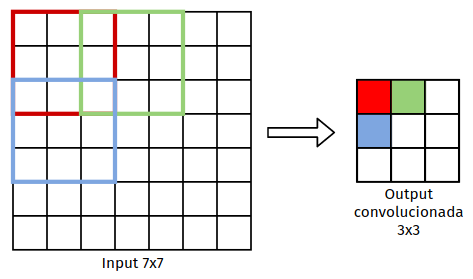
\includegraphics[width=0.6\textwidth]{tesis_44.png}
  	\caption{Convolución con \textit{stride} de 2.}
  	\label{fig:stride}
  	\end{center}
\end{figure}

\subsection{Tipos de capas}
Existen varias tipos de capas usadas \citep{rosebrock2017deep} para construir \textit{CNNs} pero las más comunes incluyen:

\begin{itemize}
	\item Convolucional (\texttt{CONV})
	\item Activación (\texttt{ACT})
	\item \textit{Pooling} (\texttt{POOL})
	\item \textit{Fully-connected} (\texttt{FC})
	\item \texttt{\textit{Dropout}} (\texttt{DO})
\end{itemize}

Apilando estas capas de una manera específica producimos una \textit{CNN}. De estos tipos de capas, \texttt{CONV} y \texttt{FC} (y en menor medida, \texttt{BN}) son las únicas capas que contienen parámetros que se aprenden durante el proceso de entrenamiento.

Las capas \texttt{ACT} y \texttt{DO} no se consideran verdaderas capas en sí mismas, pero a menudo se incluyen en los diagramas de red para que la arquitectura sea explícitamente clara.

Las capas (\texttt{POOL}), de igual importancia que \texttt{CONV} y \texttt{FC}, también se incluyen en los diagramas de red, ya que tienen un impacto sustancial en las dimensiones espaciales de un
imagen mientras se mueve a través de una \textit{CNN}.

\subsubsection{Convolución}

La capa convolucional (\texttt{CONV}) es el componente básico de una red neuronal convolucional. Los parámetros de la capa \texttt{CONV} consisten en un conjunto de $K$ \textit{kernels} entrenables, donde cada uno tiene un ancho y un alto, y casi siempre son cuadrados. 

Una capa o filtro puede tener varios \textit{kernels} que al convolucionar con el vector de entrada (que podría ser una imagen) producen mapas de características (\textit{features map}).

\begin{figure}[H]
	\begin{center}				
	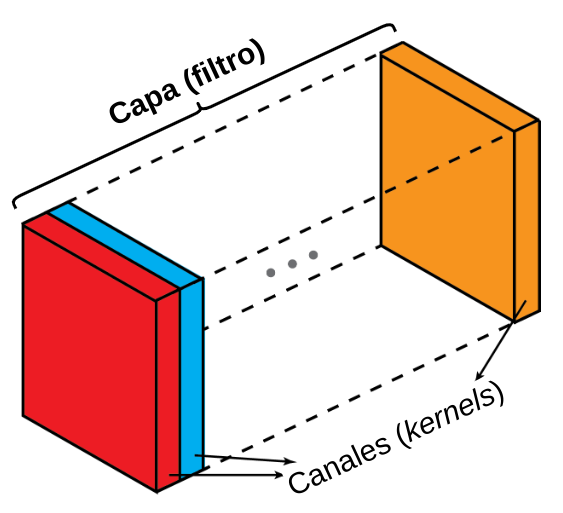
\includegraphics[width=0.45\textwidth]{layer-kernels.png}
  	\caption{Una capa está compuesta de una colección de \textit{kernels}.}
  	\label{fig:layer-kernel}
  	\end{center}
\end{figure}

La diferencia entre filtro y \textit{kernel} es un poco complicada. A veces, se usan indistintamente, lo que podría crear confusiones. Esencialmente, estos dos términos tienen una sutil diferencia. Un "\textit{kernel}" se refiere a una matriz 2D de pesos. El término "filtro" se refiere a estructuras 3D de varios \textit{kernels} apilados juntos. Para un filtro 2D, el filtro es igual que el kernel. Pero para un filtro 3D y la mayoría de las convoluciones en el aprendizaje profundo, un filtro es una colección de \textit{kernels} (fig.~\ref{fig:layer-kernel}). Cada \textit{kernel} es único, enfatizando diferentes aspectos del canal de entrada.

El funcionamiento de la capa convolucional se resume en pensar en cada uno de los $K$ \textit{kernels} deslizándose a través del vector de entrada, computando un producto de Hadamard, sumando cada uno de sus valores y luego almacenando el valor generado en un mapa 2D de activación. En la figura~\ref{fig:conv-mechanism} se puede observar una visualización de la secuencia.

\begin{figure}[H]
	\begin{center}				
	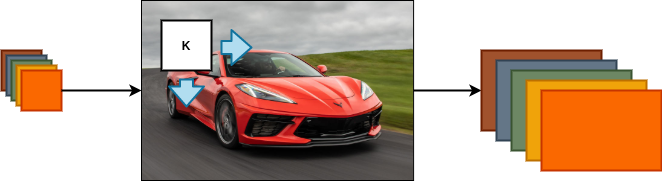
\includegraphics[width=1\textwidth]{feature-map-clean.png}
  	\caption{\textbf{Izquierda:} en cada capa convolucional de una \textit{CNN}, hay $K$ \textit{kernels} distintos. \textbf{Medio:} Cada uno de los \textit{kernels} es convolucionado con el vector de entrada. \textbf{Derecha:} Cada \textit{kernel} produce una salida 2D, llamada mapa de activación o \textit{features}.}
  	\label{fig:conv-mechanism}
  	\end{center}
\end{figure}

Luego de aplicar los $K$ filtros al vector de entrada, ahora tenemos $K \times 2D$ mapas de activación. Luego apilamos nuestro $K$ mapas de activación a través de la dimensión de profundidad de nuestra matriz para formar el volumen final de salida (figura~\ref{fig:k-maps}).

\begin{figure}[H]
	\begin{center}				
	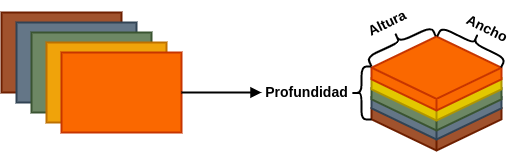
\includegraphics[width=0.8\textwidth]{k-activation-map.png}
  	\caption{Luego de obtener los $K$ mapas de activación, son apilados juntos para formar el volumen de entrada a la siguiente capa en la red.}
  	\label{fig:k-maps}
  	\end{center}
\end{figure}

Cada entrada en el volumen de salida es, por tanto, una salida de una neurona que "mira" sólo una pequeña región de la entrada. De esta manera, la red "aprende" los filtros que se activan cuando ven un tipo específico de característica en una ubicación espacial determinada en el volumen de entrada.

En las capas inferiores de la red, los filtros pueden activarse cuando ven regiones con forma de borde o de esquina. Luego, en las capas más profundas de la red, los filtros pueden activarse en presencia de características de alto nivel, como partes de la cara, la pata de un perro, el capó de un automóvil, etc.

\subsubsection{Activación}

Luego de cada capa \texttt{CONV} en una \textit{CNN}, normalmente aplicamos una función no lineal, como ReLU, ELU, etc (se ejemplifica en la figura~\ref{fig:relu-act}). Las capas \texttt{ACT} no son técnicamente "capas" (debido al hecho de que no se aprenden parámetros/pesos dentro de una capa de activación) y, a veces, se omiten en los diagramas de arquitectura de red, ya que se supone que una activación sigue inmediatamente a una convolución.

\begin{figure}[H]
	\begin{center}				
	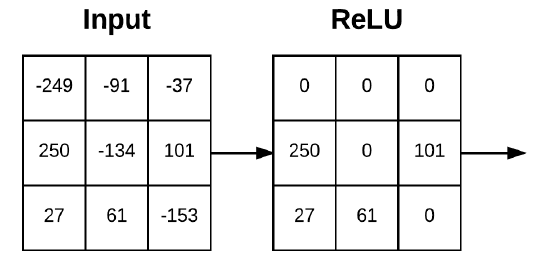
\includegraphics[width=0.65\textwidth]{tesis_47.png}
  	\caption{Un ejemplo de un volumen de entrada desplazándose a través de una \texttt{ACT} ReLU.}
  	\label{fig:relu-act}
  	\end{center}
\end{figure}

\subsubsection{\textit{Fully-connected}}
Las neuronas en las capas \texttt{FC} están totalmente conectadas a todas las activaciones de la capa anterior, como en una red neuronal \textit{feed-forward}. Siempre se ubican al final de la red.

\subsubsection{\textit{Pooling}}

Similar a la capa convolucional, la capa de \texttt{POOL} es responsable de reducir el tamaño espacial de la entidad convolucionada. Esto es para disminuir la potencia computacional requerida para procesar los datos a través de la reducción de dimensionalidad. Además, es útil para extraer características dominantes que son invariantes rotacionales y posicionales, manteniendo así el proceso de entrenamiento efectivo del modelo.

Existen dos tipos:
\begin{itemize}
	\item \textit{Max pooling} (\texttt{MPOOL}): devuelve el valor máximo de la parte de la imagen cubierta por el \textit{kernel} (figura \ref{fig:type-pooling} arriba).
	\item \textit{Average pooling} (\texttt{APOOL}): devuelve el promedio de todos los valores de la parte de la imagen cubierta por el \textit{kernel} (figura \ref{fig:type-pooling} abajo).
\end{itemize}

\begin{figure}[H]
	\begin{center}				
	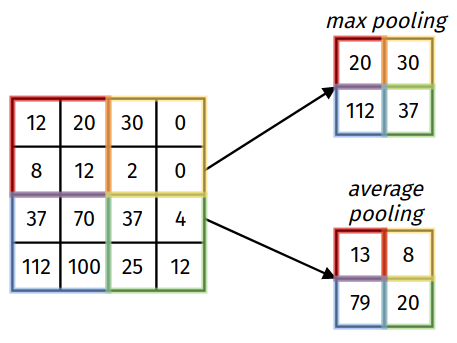
\includegraphics[width=0.5\textwidth]{tesis_45.png}
  	\caption{Tipos de \textit{pooling}.}
  	\label{fig:type-pooling}
  	\end{center}
\end{figure}

Cabe destacar que \texttt{MAXPOOL} también actúa como supresor de ruido ya que descarta las activaciones ruidosas por completo además de la reducción de dimensionalidad. Por otro lado, el \texttt{AVGPOOL} simplemente realiza la reducción de dimensionalidad como un mecanismo de supresión de ruido. Por lo tanto, podemos decir que \texttt{MAXPOOL} funciona mucho mejor que \texttt{AVGPOOL}.

\subsubsection{\textit{Batch Normalization}}

%Las capas de normalización por lotes o \textit{Batch Normalization} (\texttt{BN}), como su nombre indica, se utilizan para normalizar las activaciones de un volumen de entrada determinado antes de pasarlo a la siguiente capa de la red.

Por lo general, para entrenar una red neuronal, realizamos un preprocesamiento de los datos de entrada, por ejemplo, normalizar todos los datos para que se parezcan a una distribución normal (es decir, media cero y una varianza unitaria). Algunas razones para realizar esto puede ser prevenir la saturación temprana de funciones de activación no lineales como la función sigmoidea, asegurar que todos los datos de entrada estén en el mismo rango de valores, etc. \citep{bn}

Pero el problema aparece en las capas intermedias porque la distribución de las activaciones cambia constantemente durante el entrenamiento. Esto ralentiza el proceso de entrenamiento porque cada capa debe aprender a adaptarse a una nueva distribución en cada paso del entrenamiento. Este problema se conoce como \textbf{cambio de covariables interno}.

Podemos utilizar la normalización por lotes o \textit{Batch Normalization} (\texttt{BN}) como un método para normalizar las entradas de cada capa para así forzarlo a tener aproximadamente la misma distribución en cada paso de entrenamiento, con el fin de combatir el problema expresado anteriormente.

Durante el tiempo de entrenamiento, una capa de normalización por lotes se obtiene el promedio y la varianza del lote:

$$ \mu_{\beta} = \frac{1}{m} \sum_{i=1}^m x_i $$

$$ \sigma_{\beta}^2 = \frac{1}{m}  \sum_{i=1}^m (x_i - \mu_{\beta} ) ^2$$

Normalizamos las entradas de la capa usando las estadísticas del lote calculados previamente:

$$ \bar{x_i} = \frac{x_i - \mu_{\beta}}{\sqrt{\sigma_{\beta}^2+\epsilon}} $$

%Escalamos y \textit{shifteamos} en orden para obtener la salida de la capa:

%$$ y_i = \gamma \hat{x_i} + \beta $$

Establecemos $1e-7 \leq \epsilon \leq 0$ para evitar sacar la raíz cuadrada de cero. Aplicar esta ecuación implica que las activaciones que salen de una capa \texttt{BN} tendrán una media y una varianza unitaria aproximadamente cero (es decir, centrada en cero).
Reemplazamos el mini-lote $\mu_{\beta}$ y $\sigma_{\beta}$ con promedios de $\mu_{\beta}$ y $\sigma_{\beta}$ calculados durante el proceso de entrenamiento. Esto asegura que podemos pasar vectores a través de nuestra red y aún así obtener predicciones precisas sin ser sesgados por $\mu_{\beta}$ y $\sigma_{\beta}$ del mini-lote final pasado a través de la red en el momento del entrenamiento. 

La \texttt{BN} también tiene el beneficio adicional de ayudar a "estabilizar" el entrenamiento, lo que permite una mayor variedad de tasas de aprendizaje y fortalezas de regularización. Esto no alivia la necesidad de ajustar estos parámetros, por supuesto, pero le facilitará la vida al hacer que la tasa de aprendizaje y la regularización sean menos volátiles y más fáciles de ajustar. También tenderá a notar pérdidas finales más bajas y una curva de pérdida más estable en sus redes.

\subsubsection{\textit{Dropout}}
El \textit{dropout} (\texttt{DO}) es en realidad una forma de regularización que tiene como objetivo ayudar a prevenir el sobreajuste aumentando la precisión de las pruebas, quizás a expensas de la precisión del entrenamiento. \citep{rosebrock2017deep}

La razón está en reducir el sobreajuste alterando de forma explicita la arquitectura de la red en tiempo de entrenamiento. La desconexión aleatoria de las conexiones garantiza que ningún nodo de la red sea responsable de la activación cuando se le presenta un patrón determinado. El \texttt{DO} garantiza que haya múltiples nodos redundantes que se activarán cuando se les presenten entradas similares (lo que a su vez ayuda a que nuestro modelo a generalizar).

\begin{figure}[H]
	\begin{center}				
	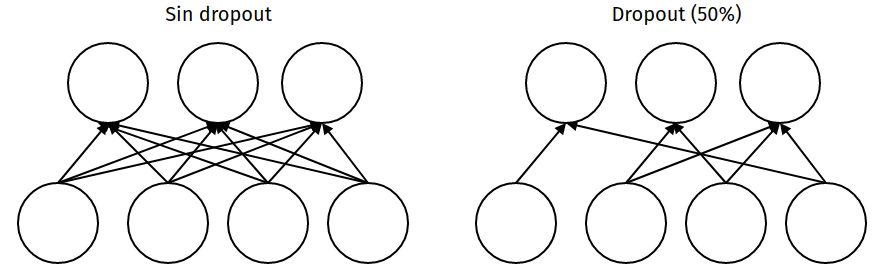
\includegraphics[width=1\textwidth]{tesis_46.png}
  	\caption{\textbf{Izquierda:} Dos capas \texttt{FC} sin \texttt{DO}. \textbf{Derecha:} Las mismas dos capas luego de realizar \textit{dropout} sobre la mitad de las conexiones.}
  	\label{fig:type-pooling}
  	\end{center}
\end{figure}

\subsection{\textit{WaveNet} y capas convolucionales causales dilatadas}

\textit{WaveNet} es una red neuronal profunda para generar audio muestra a muestra. La arquitectura de este modelo permite aprovechar las eficiencias de las capas de convolución al mismo tiempo que alivia el desafío de aprender las dependencias a largo plazo en una gran cantidad de pasos de tiempo (más de 1000) \citep{wavenet2}.

En el núcleo de \textit{WaveNet} se encuentra la \textbf{capa de convolución causal dilatada} (figura~\ref{fig:causal-conv}), que le permite tratar adecuadamente el orden temporal y manejar las dependencias a largo plazo sin una explosión en la complejidad del modelo. \citep{wavenet}

\begin{figure}[H]
	\begin{center}				
	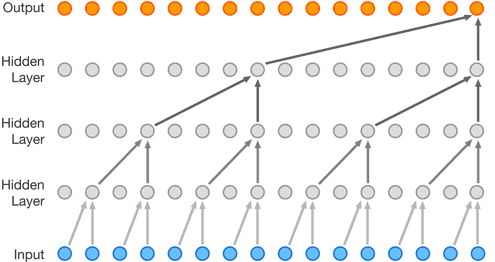
\includegraphics[width=0.8\textwidth]{causal-conv.png}
  	\caption{Paso de la información a través de la capa de convolución causal dilatada.}
  	\label{fig:causal-conv}
  	\end{center}
\end{figure}

En una capa de convolución unidimensional tradicional, deslizamos un filtro de pesos a través de una serie de entrada, aplicándolo secuencialmente a las regiones (generalmente superpuestas) de la serie. Pero cuando utilizamos el historial de una serie temporal para predecir su futuro, debemos tener cuidado. A medida que formamos capas que eventualmente conectan los pasos de entrada a las salidas, debemos asegurarnos de que las entradas no influyan en los pasos de salida que los siguen a tiempo. De lo contrario, estaríamos usando el futuro para predecir el pasado, lo que sería hacer trampa.

Para asegurarnos de no hacer trampa de esta manera, ajustamos nuestro diseño de convolución para prohibir explícitamente que el futuro influya en el pasado. En otras palabras, solo permitimos que las entradas se conecten a salidas de pasos de tiempo futuros en una estructura \textbf{causal}, como se muestra a continuación en una visualización del documento WaveNet. En la práctica, esta estructura 1D causal es fácil de implementar \textit{shifteando} las salidas convolucionales tradicionales en varios pasos de tiempo.

\begin{figure}[H]
	\begin{center}				
	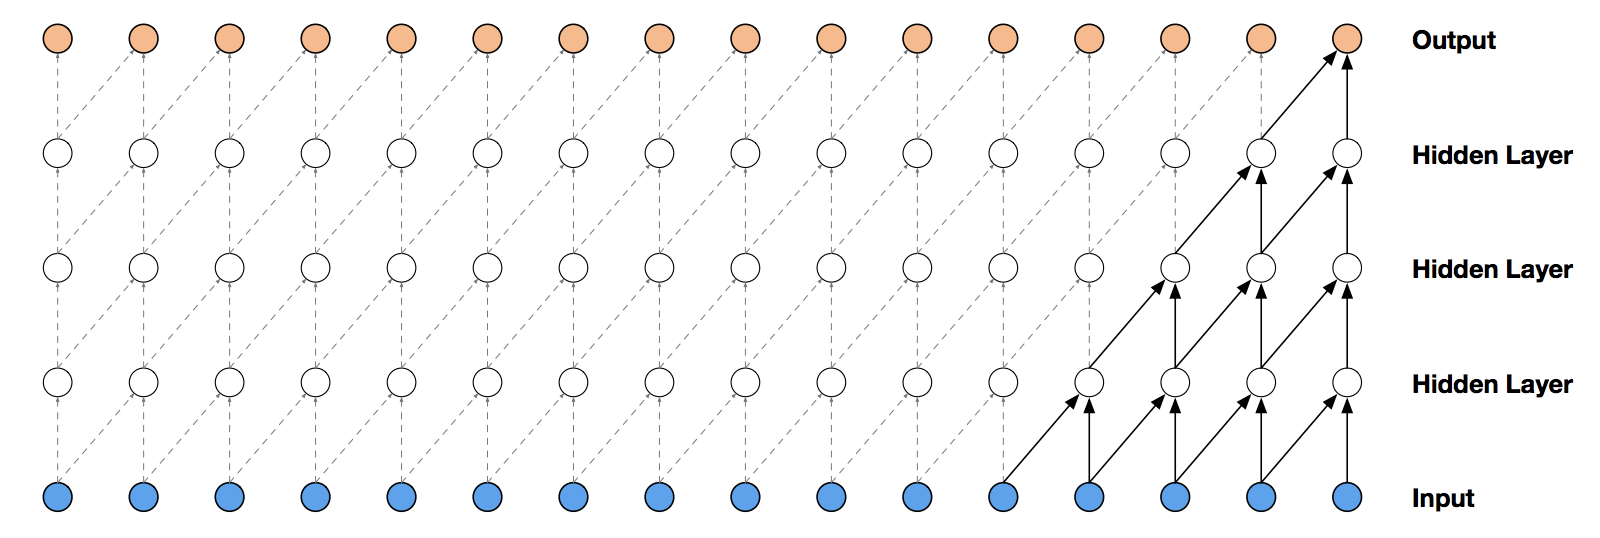
\includegraphics[width=1\textwidth]{stackcausal-conv.png}
  	\caption{Visualización de una pila de capas causales convoluciones.}
  	\label{fig:stackcausal-conv}
  	\end{center}
\end{figure}

Las convoluciones causales proporcionan la herramienta adecuada para manejar el flujo temporal, pero necesitamos una modificación adicional para manejar adecuadamente las dependencias a largo plazo. En la figura \ref{fig:stackcausal-conv} de convolución causal simple, puede ver que solo los 5 pasos de tiempo más recientes pueden influir en la salida resaltada. De hecho, necesitaríamos una capa adicional por paso de tiempo para llegar más atrás en la serie (para usar la terminología adecuada, para aumentar el \textbf{campo receptivo de la salida}). Con una serie de tiempo que tiene una gran cantidad de pasos, el uso de convoluciones causales simples para aprender de toda la historia rápidamente haría un modelo demasiado complejo computacional y estadísticamente.

\begin{figure}[H]
	\begin{center}				
	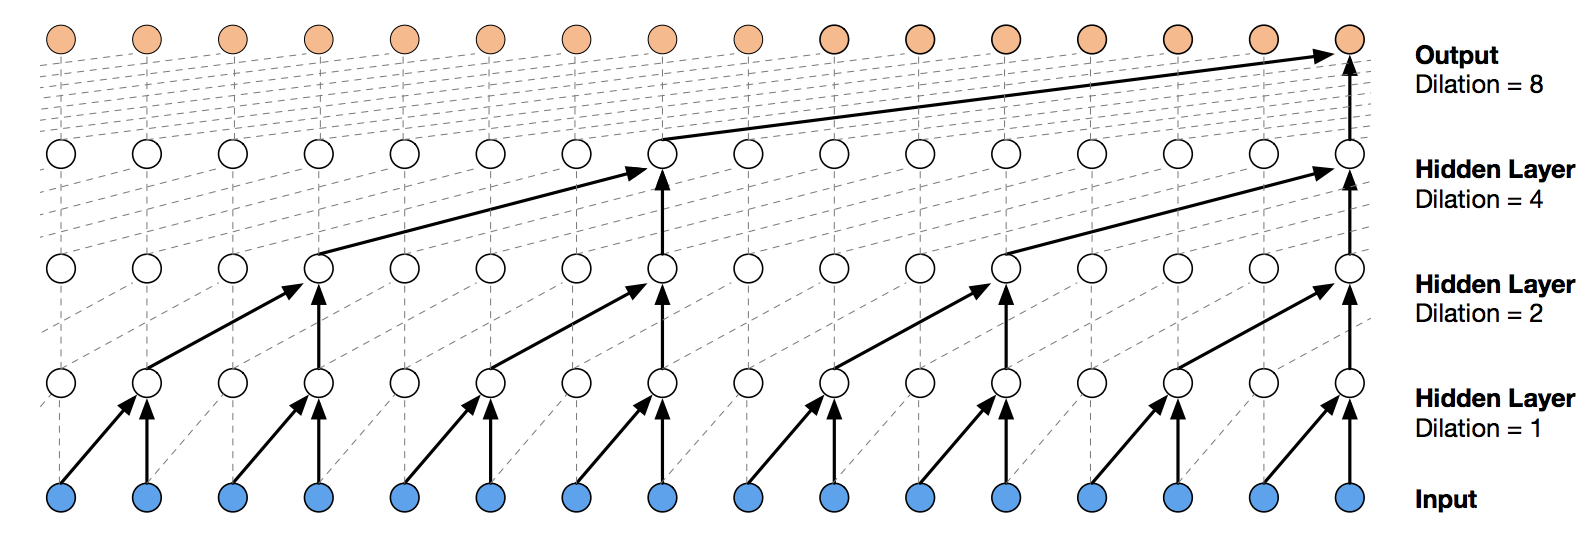
\includegraphics[width=1\textwidth]{dilated-conv.png}
  	\caption{Visualización de una pila de capas causales convoluciones dilatadas.}
  	\label{fig:dilated-conv}
  	\end{center}
\end{figure}

En lugar de cometer ese error, \textit{WaveNet} utiliza \textbf{convoluciones dilatadas}, que permiten que el campo receptivo aumente exponencialmente en función de la profundidad de la capa de convolución. 

En una capa de convolución dilatada, los filtros no se aplican a las entradas de una manera secuencial simple, sino que omiten una entrada de tasa de dilatación constante entre cada una de las entradas que procesan, como en el diagrama \textit{WaveNet} a continuación. Al aumentar la tasa de dilatación multiplicativamente en cada capa (por ejemplo, 1, 2, 4, 8,…), podemos lograr la relación exponencial entre la profundidad de la capa y el tamaño del campo receptivo que deseamos. 

En la figura~\ref{fig:dilated-conv}, puede ver cómo ahora solo necesitamos 4 capas para conectar los 16 valores de la serie de entrada a la salida resaltada (digamos, el valor de paso de tiempo 17). Por extensión, cuando se trabaja con una serie de tiempo diaria, se puede capturar más de un año de historia con solo 9 capas de convolución dilatadas de esta forma.

\section{Redes neuronales recurrentes}
Anteriormente hemos visto cómo las redes neuronales o convolucionales nos permiten clasificar un dato, por ejemplo una palabra, un sonido, o una imagen, pero tienen un inconveniente, y es que cuando tenemos una secuencia de datos, por ejemplo una secuencia de palabras, o una conversación, o una secuencia de imágenes, es decir un vídeo, este tipo de arquitecturas no pueden procesar ese tipo de datos. 

Las Redes Neuronales Recurrentes \textit{(RNN)} \citep{karpathy:rnn} resuelven este inconveniente, porque son capaces de procesar diferentes tipos de secuencias, como textos, conversaciones, vídeos, música, y además de eso no sólo clasifican los datos como lo hacen las redes neuronales o convolucionales, sino que también están en capacidad de generar nuevas secuencias.

Si a una red neuronal o convolucional se le presenta una imagen o una palabra, con el entrenamiento adecuado estas arquitecturas lograrán clasificar un sinnúmero de datos, logrando a la vez una alta precisión. 

Pero, ¿qué sucede si en lugar de una única imagen o palabra se introduce a la red una secuencia de imágenes, es decir un vídeo, o una secuencia de palabras (una conversación)? En este caso en ninguna de estas redes será capaz de procesar los datos por dos motivos:
\begin{itemize}
	\item Estas arquitecturas están diseñadas para que los datos de entrada y de salida siempre tengan el mismo tamaño; sin embargo, un vídeo o una conversación se caracterizan por ser un tipo de datos con un tamaño variable: una cantidad variable de "frames"
en el caso del vídeo o una cantidad variable de palabras en el caso de la conversación. 
	\item En un vídeo o en una conversación los datos están \textbf{correlacionados}, esto quiere decir que la siguiente palabra pronunciada o la siguiente imagen en la secuencia de vídeo dependerá de la palabra o imagen anterior. E incluso estas palabras e imágenes estarán relacionadas con aquellas que se presenten más adelante en la secuencia y una \textit{NN} ó \textit{CNN} no está en capacidad de analizar la relación entre varias palabras o imágenes de la secuencia.
\end{itemize}

Una secuencia es una serie de datos que siguen un orden específico y tienen únicamente significado cuando se analizan en conjunto y no de manera individual. Dichos datos, analizados de forma individual o en un orden diferente, carecen de significado. Es evidente que una secuencia no tiene un tamaño predefinido pues no podemos saber con antelación el número de datos. 

Las \textit{RNN} resuelven los inconvenientes expresados anteriormente, pues pueden procesar tanto a la entrada como a la salida secuencias sin importar su tamaño, y además teniendo en cuenta la correlación existente entre los diferentes elementos de esa secuencia.

Para ello este tipo de redes usan el concepto de recurrencia: para generar la salida, que también se conoce como activación, la red usa no sólo la entrada actual sino la activación generada en la iteración previa. En pocas palabras, las redes neuronales recurrentes usan un cierto tipo de memoria para generar la salida deseada. 

\subsection{Arquitecturas} \label{rnnarchitecture}
Existen diversas arquitecturas disponibles para estas redes como observamos en la Figura~\ref{fig:rnnarch} \cite{karpathy:rnn}, donde cada rectángulo es un vector y cada fecha representa funciones. Los vectores de entrada están en rojo, los vectores de salida están en azul y los vectores verdes mantienen el estado de la \textit{RNN}.

\begin{figure}[H]
	\begin{center}				
	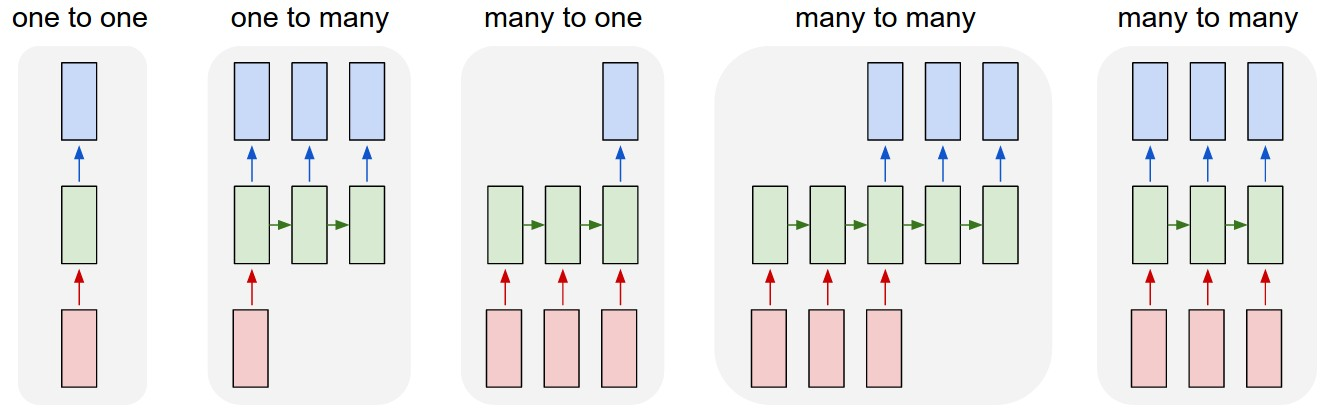
\includegraphics[width=1\textwidth]{rnnarch.jpg}
  	\caption{Tipos de arquitecturas para una \textit{RNN}.}
  	\label{fig:rnnarch}
  	\end{center}
\end{figure}

\textbf{\textit{One-to-one}}
Modo de procesamiento vanilla \textit{i.e.} sin \textit{RNN}, desde una entrada de tamaño fijo a una salida de tamaño fijo, por ejemplo la clasificación de imágenes.

\textbf{\textit{One-to-many}}

La entrada es un único dato y la salida es una secuencia. Un ejemplo de esta arquitectura es el "\textit{image captioning}" en donde la entrada es una y la salida es una secuencia de caracteres, un texto, que describe el contenido de la imagen. 

\textbf{\textit{Many-to-one}}

La entrada es una secuencia y la salida es por ejemplo una categoría. Un ejemplo de esto es la clasificación de sentimientos, en donde por ejemplo la entrada es un texto que contiene una crítica a una película y la salida es una categoría indicando si la película le gustó a la persona o no.

\textbf{\textit{Many-to-many}}
Tanto la entrada como a la salida se tienen secuencias. La primer figura se refiere a \textit{RNN} utilizadas en traductores automáticos: en este caso la secuencia de salida no se genera al mismo tiempo que la secuencia de entrada pues para poder traducir por ejemplo una frase al español se requiere primero conocer la totalidad del texto en inglés. Y desde luego, en esta misma arquitectura podemos encontrar los conversores de voz a texto o texto a voz.
La segunda figura se refiere a secuencias sincronizadas de entrada y salida, por ejemplo clasificación de vídeo donde deseamos etiquetar cada fotograma.

Como era de esperar, el régimen secuencial de operación es mucho más poderoso en comparación con las redes fijas que están condenadas desde el principio por un número fijo de pasos computacionales y, por lo tanto, también es más provechoso a la hora de construir sistemas más inteligentes. 

Además, las \textit{RNN} combinan el vector de entrada con su vector de estado con una función fija (pero aprendida) para producir un nuevo vector de estado. En términos de programación, esto puede interpretarse como ejecutar un programa fijo con ciertas entradas y algunas variables internas. Visto de esta manera, los RNN esencialmente describen programas.

\textbf{Si entrenar redes neuronales es optimización sobre funciones, entrenar redes recurrentes es optimización sobre programas.}

\subsection{Funcionamiento}

Consideremos la Figura~\ref{fig:rnnunit} \citep{olahlstm}, aquí podemos observar como se define de manera gráfica una unidad funcional de una \textit{RNN} denominada $A$, que toma una entrada $x_t$ y genera un valor $h_t$.

\begin{figure}[H]
	\begin{center}				
	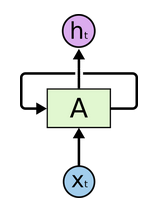
\includegraphics[width=0.2\textwidth]{tesis_27.png}
  	\caption{Unidad funcional de \textit{RNN}.}
  	\label{fig:rnnunit}
  	\end{center}
\end{figure}

El \textit{loop} de A permite que la información pase de un paso de la red al siguiente.

Una red neuronal recurrente se puede considerar como múltiples copias de la misma red, cada una de las cuales pasa un mensaje a un sucesor. si desenrollamos el ciclo podemos representar la \textit{RNN} a través del eje del tiempo, como se muestra en la Figura~\ref{fig:rnnunrolled}.

\begin{figure}[H]
	\begin{center}
	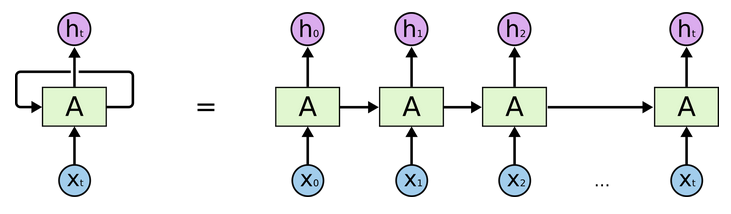
\includegraphics[width=0.9\textwidth]{tesis_28.png}
  	\caption{Una \textit{RNN} desenrrollada.}
  	\label{fig:rnnunrolled}
  	\end{center}
\end{figure}

Esta naturaleza en cadena revela que las redes neuronales recurrentes están íntimamente relacionadas con secuencias y listas.

En su esencia una \textit{RNN} se parece demasiado a una \textit{FFNN}, excepto que también tiene conexiones hacía atrás.
La \textit{RNN} más simple posible es la que mostramos en la figura 


\begin{figure}[H]
	\begin{center}				
	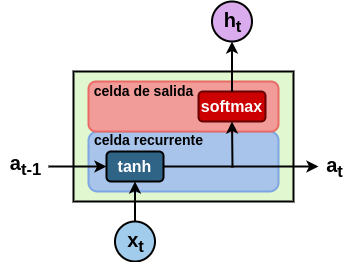
\includegraphics[width=0.5\textwidth]{rnnunitv2.png}
  	\caption{Unidad funcional \textit{RNN} detallada.}
  	\label{fig:rnnunitv2}
  	\end{center}
\end{figure}

En la Figura~\ref{fig:rnnunitv2} se observa que en cada instante de tiempo la red tiene realmente dos entradas y dos salidas. Las entradas son el dato actual, $x_t$ y la activación anterior, $a_{t-1}$, mientras que las salidas son la predicción actual, $y_t$, y la activación actual, $a_t$. Esta activación también recibe el nombre de \textit{hidden state} o estado oculto.

Se define:

$$ a_{t} = tanh(W_{aa}a_{t-1}+W_{ax}x_t+b_a) $$
$$ h_t = softmax(W_{ya}a_t + b_y) $$

Donde:

$ W_{ax}:$ matriz de pesos multiplicando la entrada.

$ W_{aa}:$ matriz de pesos multiplicando el estado oculto.

$ W_{ya}:$ matriz de pesos que relaciona el estado oculto a la salida.

$b_a:$ bias.

$b_y:$ bias que relaciona el estado oculto a la salida.

Es posible entrenar una RNN con una gran cantidad de texto y le pediremos que modele la distribución de probabilidad del siguiente carácter en la secuencia dada una secuencia de caracteres anteriores. Esto nos permitirá generar texto nuevo, de a un carácter a la vez.

Como ejemplo práctico, suponga que solo tenemos un vocabulario de cuatro letras posibles \texttt{helo} y queremos entrenar a un RNN en la secuencia de entrenamiento \texttt{hello}. Esta secuencia de entrenamiento es de hecho una fuente de 4 ejemplos de entrenamiento separados: 
\begin{enumerate}
	\item La probabilidad de \texttt{e} probablemente debería estar dado el contexto de \texttt{h}.
	\item \texttt{l} debería estar probablemente en el contexto de \texttt{he}.
	\item \texttt{l} probablemente también debería ser dado el contexto de \texttt{hel}.
	\item  Y finalmente \texttt{o} debería ser probablemente dado el contexto de \texttt{hell}.
\end{enumerate}

Concretamente, codificaremos cada carácter en un vector usando la codificación \textit{1-of-k} (es decir, todo cero excepto uno en el índice del carácter en el vocabulario) y los introduciremos en el RNN uno a la vez con el función \texttt{step}. Luego observaremos una secuencia de vectores de salida de 4 dimensiones (una dimensión por carácter), que interpretamos como la confianza que el RNN asigna actualmente a cada carácter que sigue en la secuencia. 

\begin{figure}[H]
	\begin{center}				
	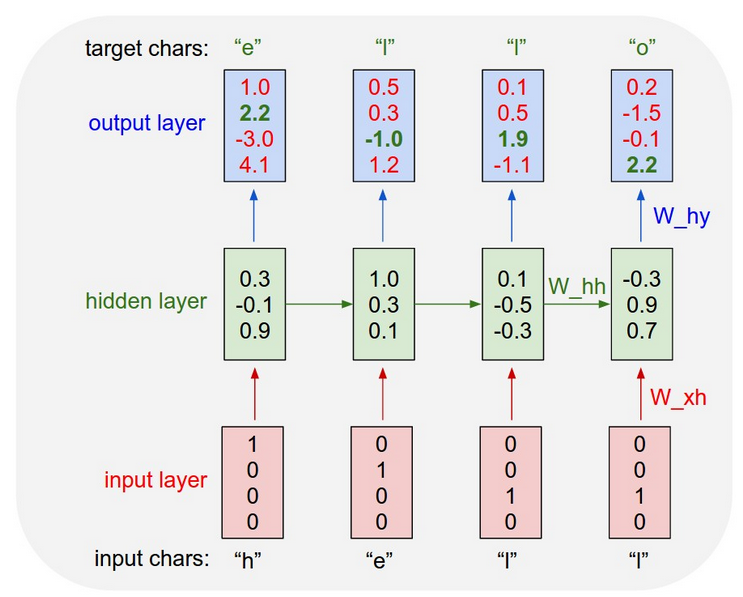
\includegraphics[width=0.6\textwidth]{tesis_29.png}
  	\caption{Unidad funcional \textit{RNN} detallada.}
  	\label{fig:rnnexample}
  	\end{center}
\end{figure}

En la Fig.~\ref{fig:rnnexample} observamos un ejemplo de \textit{RNN} con capas de entrada y salida de 4 dimensiones y una capa oculta de 3 unidades (neuronas). Las activaciones en el pase hacia adelante cuando el \textit{RNN} recibe los caracteres \texttt{"hell"} como entrada. La capa de salida contiene los pesos que el \textit{RNN} asigna al siguiente carácter (el vocabulario es \texttt{"h, e, l, o"}); Queremos que los números verdes sean altos y los números rojos bajos.

Por ejemplo, vemos que en el primer paso de tiempo cuando el \textit{RNN} vio el carácter \texttt{"h"} asignó un peso de $1.0$ a la siguiente letra que era \texttt{"h"}, $2.2$ a la letra \texttt{"e"}, $-3.0$ a \texttt{"l"} y $4.1$ a "o". Dado que en nuestros datos de entrenamiento (la cadena \texttt{"hello"}) el siguiente carácter correcto es \texttt{"e"}, nos gustaría aumentar su peso (verde) y disminuir los pesos de todas las demás letras (rojo). 

De manera similar, tenemos un carácter objetivo deseado en cada uno de los 4 pasos de tiempo a los que nos gustaría que la red le asignara una mayor confianza. Dado que el \textit{RNN} consta completamente de operaciones diferenciables, podemos ejecutar el algoritmo de \textit{back-propagaton} para averiguar en qué dirección debemos ajustar cada uno de sus pesos para aumentar los pesos de los objetivos correctos. 

Luego podemos realizar una actualización de parámetros, que empuja cada peso una pequeña cantidad en esta dirección de gradiente. Si tuviéramos que alimentar las mismas entradas al RNN después de la actualización del parámetro, encontraríamos que las puntuaciones de los caracteres correctos (por ejemplo, "e" en el primer paso de tiempo) serían ligeramente más altas (por ejemplo, $2.3$ en lugar de $2.2$), y los pesos de los caracteres incorrectos serían ligeramente inferiores.

Luego, repetimos este proceso una y otra vez hasta que la red converge y sus predicciones son finalmente consistentes con los datos de entrenamiento en el sentido de que los caracteres correctos siempre se predicen a continuación.

\subsection{Entrenamiento}
Para entrenar una \textit{RNN}, el truco simplemente es desenrrollarla a través del tiempo y simplemente usar \textit{backpropagation} (estrategia que recibe el nombre de \textit{backpropagation} a través del tiempo (\textit{BPTT})) como observamos en la Fig.~\ref{fig:BPTT} \citep{geron}.

\begin{figure}[H]
	\begin{center}				
	\includegraphics[width=0.8\textwidth]{tesis_40.png}
  	\caption{\textit{Backpropagation} a través del tiempo.}
  	\label{fig:BPTT}
  	\end{center}
\end{figure}

Primero realizamos una pasada hacía adelante a través de la red desenrollada (representada en la figura por las flechas punteadas). 

Luego la secuencia de salida es evaluada utilizando una función de costo $C(Y_{(0)}, Y_{(1)}, \dots, Y_{(T)})$ (donde $T$ es el paso máximo de tiempo). Notemos que la función de coste puede ignorar algunas salidas en función de lo que necesitemos como se muestra en la Fig.~\ref{fig:BPTT}.
Los gradientes de esa función de costo luego son propagados hacía atrás a través de la red desenrrollada (representada a través de las líneas sólidas).

Finalmente los parámetros del modelo son actualizadas usando los gradientes calculados por \textit{BPTT}. Notar que los gradientes fluyen hacía atrás a través de todas las salidas utilizadas por la función de costo, no solamente a través de la salida final (notar que en el ejemplo no fluye a través de $Y_{(0)}$ e $Y_{(1)}$).

\subsection{Desvanecimiento del gradiente}

Otra forma de alimentar una \textit{RNN} podría ser a través de las palabras individuales de una oración, dado que esto se realiza de forma secuencial, debemos proveerle de una palabra a la vez.

En el ejemplo de la Fig.~\ref{fig:rnnvanishing1} intentaremos predecir la intención del usuario tomando como entrada la oración \texttt{"What time is it?"}. \citep{phi:rnn}.

\begin{figure}[H]
	\begin{center}				
	\includegraphics[width=0.6\textwidth]{vanishing1.png}
  	\caption{\textit{RNN} siendo alimentada con las palabras de la oración.}
  	\label{fig:rnnvanishing1}
  	\end{center}
\end{figure}

\begin{enumerate}
	\item Inicializa sus capas de red y el estado oculto inicial. La forma y dimensión del estado oculto dependerá de la forma y dimensión de su \textit{RNN}.
	\item Luego recorre sus entradas, pasa la palabra y el estado oculto al \textit{RNN}.
	\item El \textit{RNN} devuelve la salida y un estado oculto modificado.
	\item Continúas repitiendo hasta que te quedas sin palabras.
	\item Por último, pasa la salida a la capa de \textit{feedforward} y devuelve una predicción (Fig.~\ref{fig:rnnvanishing2}).
\end{enumerate}

\begin{figure}[H]
	\begin{center}				
	\includegraphics[width=0.6\textwidth]{vanishing2.png}
  	\caption{Predicción de la \textit{RNN}.}
  	\label{fig:rnnvanishing2}
  	\end{center}
\end{figure}

Pero prestemos atención a la Fig.~\ref{fig:rnnvanishing3}. Es posible que haya notado la extraña distribución de colores en los estados ocultos. Eso es para ilustrar un problema con los \textit{RNN} conocido como memoria a corto plazo.

\begin{figure}[H]
	\begin{center}				
	\includegraphics[width=0.2\textwidth]{vanishin3.png}
  	\caption{Estado oculto final de la \textit{RNN}.}
  	\label{fig:rnnvanishing3}
  	\end{center}
\end{figure}

La memoria a corto plazo es causada por el infame problema del desvanecimiento del gradiente, que también prevalece en otras arquitecturas de redes neuronales. A medida que el RNN procesa más pasos, tiene problemas para retener información de los pasos anteriores. 

Como puede ver, la información de la palabra \texttt{"What"} y \texttt{"time"} es casi inexistente en el último paso. La memoria a corto plazo y el desvanecimiento del gradiente se deben a la naturaleza del algoritmo de \textit{back-propagation}.

Al hacer \textit{back-propagation}, cada nodo de una capa calcula su gradiente con respecto a los efectos de los gradientes, en la capa anterior. Entonces, si los ajustes a las capas anteriores son pequeños, los ajustes a la capa actual serán aún más pequeños. 

\begin{figure}[H]
	\begin{center}				
	\includegraphics[width=0.25\textwidth]{vanishing4.png}
  	\caption{Desvanecimiento del gradiente desde las capas superiores a las inferiores.}
  	\label{fig:rnnvanishing4}
  	\end{center}
\end{figure}

Es posible pensar en cada paso de tiempo en una \textit{RNN} como una capa y para entrenarla se usa \textit{back-propagation} a través del tiempo. Los valores del gradiente se reducirán exponencialmente a medida que se propaga a través de cada paso de tiempo.

\begin{figure}[H]
	\begin{center}				
	\includegraphics[width=0.6\textwidth]{vanishing5.png}
  	\caption{El gradiente se achica a medida que se propaga hacia atrás en el tiempo.}
  	\label{fig:rnnvanishing5}
  	\end{center}
\end{figure}

Nuevamente, el gradiente se utiliza para realizar ajustes en los pesos de las redes neuronales, lo que le permite aprender. Pequeños gradientes significan pequeños ajustes. Eso hace que las capas tempranas no aprendan.

Debido a los gradientes que desaparecen, la \textit{RNN} no aprende las dependencias de largo alcance en los pasos de tiempo. Eso significa que existe la posibilidad de que las palabras \texttt{"What"} y \texttt{"time"} no se consideren al intentar predecir la intención del usuario. Entonces, la red tiene que hacer la mejor suposición con \texttt{"is it?"}. Eso es bastante ambiguo y sería difícil incluso para un humano. Por lo tanto, no poder aprender en pasos de tiempo anteriores hace que la red tenga una memoria a corto plazo.

\subsection{Tipos de \textit{RNNs}}
Para mitigar la memoria a corto plazo, se crearon dos redes neuronales recurrentes especializadas. Las redes denominadas \textit{Long Short-Term Memory} o \textit{LSTM} para abreviar. Las otras se denominan \textit{Gated Recurrent Units} o \texttt{GRU}.

\subsubsection{LSTM}
Los \texttt{LSTM} y \texttt{GRU} funcionan esencialmente como los \textit{RNN}, pero son capaces de aprender las dependencias a largo plazo mediante mecanismos llamados "puertas". Estas puertas son diferentes operaciones de tensor que pueden aprender qué información agregar o quitar al estado oculto. Debido a esta capacidad, la memoria a corto plazo es un problema menor para ellos. \citep{olahlstm}

Si consideramos la celda \texttt{LSTM} como una caja negra, aparenta ser idéntica a una \textit{RNN} excepto que su estado se divide en dos vectores: $h_{(t)}$ y $c_{(t)}$ ("c" se mantiene por celda). Es posible pensar a $h_{(t)}$ como un estado de corto plazo y a $c_{(t)}$ como un estado de largo plazo.

\begin{figure}[H]
	\begin{center}				
	\includegraphics[width=1\textwidth]{lstmcell5.png}
  	\caption{Celda \texttt{LSTM}.}
  	\label{fig:lstmcell}
  	\end{center}
\end{figure}

El diagrama completo del \texttt{LSTM} lo podemos observar en la Fig.\ref{fig:lstmcell}, pero vamos a ir paso a paso analizando cada una de las partes que lo componen.

La clave de los \texttt{LSTM} es el estado de la celda, la línea horizontal que atraviesa la parte superior de la Fig.~\ref{fig:lstm1}. El estado de la celda es como una cinta transportadora. Corre directamente a lo largo de toda la cadena, con solo algunas interacciones lineales menores. Es muy fácil que la información fluya sin cambios.

\begin{figure}[H]
	\begin{center}				
	\includegraphics[width=1\textwidth]{lstm1.png}
  	\caption{Celda de estado.}
  	\label{fig:lstm1}
  	\end{center}
\end{figure}

El \texttt{LSTM} tiene la capacidad de eliminar o agregar información al estado de la celda, regulada cuidadosamente por estructuras llamadas puertas. Las puertas son una forma de dejar pasar información opcionalmente. Están compuestos por una capa de red neuronal sigmoidea y una operación de multiplicación.

La capa sigmoidea genera números entre $0$ y $1$, que describen cuánto de cada componente debe dejarse pasar. Un valor de $0$ significa "no dejar pasar nada", mientras que un valor de $1$ significa "dejar pasar todo". Un \texttt{LSTM} tiene tres de estas puertas para proteger y controlar el estado de la celda.

El primer paso es decidir qué información vamos a eliminar del estado de la celda. Esta decisión la toma una capa sigmoidea llamada \textbf{puerta del olvido} (Fig.~\ref{fig:lstm2}). Examina $h_{t-1}$ y $x_t$, y genera un número entre $0$ y $1$ para cada número en el estado de celda $C_{t-1}$. Un $1$ representa "mantener esto completamente", mientras que un $0$ representa "deshacerse de esto por completo".

\begin{figure}[H]
	\begin{center}				
	\includegraphics[width=0.5\textwidth]{lstm2.png}
  	\caption{Puerta del olvido.}
  	\label{fig:lstm2}
  	\end{center}
\end{figure}

Por tanto la puerta del olvido queda representada por la siguiente ecuación:

$$f_{(t)} = \sigma (W_{xf}x_{(t)} + W_{hf}h_{(t-1)} + b_f)$$

El siguiente paso es decidir qué nueva información almacenaremos en el estado de la celda. Esto tiene dos partes. 

\begin{figure}[H]
	\begin{center}				
	\includegraphics[width=0.5\textwidth]{lstm3.png}
  	\caption{Puerta de entrada.}
  	\label{fig:lstm3}
  	\end{center}
\end{figure}

Una capa sigmoidea llamada \textbf{puerta de entrada} (Fig~\ref{fig:lstm3}) decide qué valores actualizaremos.

$$i_{(t)}=\sigma(W_{xi}x_{(t)} + W_{hi}h_{(t-1)} + b_i)$$

A continuación, una capa $tanh$ crea un vector de nuevos valores candidatos, que podrían agregarse al estado. 

$$g_{(t)}=tanh(W_{xg}x_{(t)}+W_{hg}h_{(t-1)}+b_g)$$


En el siguiente paso, combinaremos estos dos para crear una actualización del estado.

Ahora es el momento de actualizar el estado de la celda anterior, $C_{(t-1)}$, al nuevo estado de la celda $C_{(t)}$. Los pasos anteriores ya decidieron qué hacer, solo tenemos que hacerlo realmente.

\begin{figure}[H]
	\begin{center}				
	\includegraphics[width=0.5\textwidth]{lstm4.png}
  	\caption{Actualización de la celda.}
  	\label{fig:lstm4}
  	\end{center}
\end{figure}

Multiplicamos el estado anterior por $f_{(t)}$, olvidando las cosas que decidimos olvidar antes. Luego le sumamos $i_{(t)} \otimes g_{(t)}$. Estos son los nuevos valores candidatos, escalados según cuánto decidimos actualizar cada valor de estado.

$$C_{(t)} = f_{(t)} \otimes C_{(t-1)} + i_{(t)} \otimes g_{(t)}$$

\begin{figure}[H]
	\begin{center}				
	\includegraphics[width=0.5\textwidth]{lstm5.png}
  	\caption{Puerta de salida.}
  	\label{fig:lstm5}
  	\end{center}
\end{figure}

Finalmente, tenemos que decidir qué vamos a producir. Esta salida se basará en el estado de nuestra celda, pero será una versión filtrada. Primero, ejecutamos una capa sigmoidea que denominaremos \textbf{puerta de salida} que decide qué partes del estado de la celda vamos a generar. Luego, colocamos el estado de la celda a través de $tanh$ (para presionar los valores entre $-1$ y $1$) y lo multiplicamos por la salida de la puerta, de modo que solo produzcamos las partes que decidimos.

$$ o_{(t)}=\sigma (W_{xo}x_{(t)} + W_{ho}h_{(t-1)} + b_o) $$

$$ h_{(t)}=o_{(t)} \otimes tanh(C_{(t)})$$

Pasando en limpio observando nuevamente la Fig.~\ref{fig:lstmcell}, tendremos nuestro vector de entradas $x_{(t)}$ y el estado anterior de corto plazo $h_{(t-1)}$ que alimenta 4 capas \texttt{FC}. Cada una de ellas sirve a un propósito diferente \citep{geron}:

\begin{itemize}
	\item La capa principal es la que genera $g_{(t)}$. Tiene la función habitual de analizar las entradas actuales $x_{(t)}$ y el estado anterior (a corto plazo) $h_{(t-1)}$. En una celda básica \textit{RNN}, no hay nada más que esta capa, y su salida va directamente hacia $y_{(t)}$ y $h_{(t)}$. Por el contrario, en una celda \texttt{LSTM}, la salida de esta capa no sale directamente, sino que se almacena parcialmente en el estado a largo plazo.
	\item Las otras tres capas son controladores de puerta. Dado que usan la función de activación sigmoidea, sus salidas van entre 0 y 1. Sus salidas se alimentan a operaciones de multiplicación elemento a elemento (también conocido como producto de Hadamard \citep{hadamard}), por lo que si generan ceros, cierran la puerta, y si generan 1 la abre. Específicamente:
	\begin{itemize}
	\item La puerta de olvido (controlada por $f_{(t)}$) controla qué partes del estado a largo plazo $C_{(t-1)}$ deben borrarse.
	\item La puerta de entrada (controlada por $i_{(t)}$) controla qué partes de $g_{(t)}$ deben agregarse al estado a largo plazo.
	\item La puerta de salida (controlada por $o_{(t)}$) controla qué partes del estado a largo plazo deben leerse y generarse en este paso de tiempo (tanto en $h_{(t)}$ como en $y_{(t)}$).
	\end{itemize}
\end{itemize}

En resumen, una celda \texttt{LSTM} puede aprender a reconocer una entrada importante (ese es el papel de la puerta de entrada), almacenarla en el estado a largo plazo, aprender a preservarla durante el tiempo que sea necesario (ese es el papel de la puerta del olvido) y aprender a extraerla siempre que sea necesario.

\subsubsection{GRU}

Otra variante popular es la celda \texttt{GRU} (Unidad Recurrente Cerrada, \textit{Gated Recurrent Unit)}. \citep{olahlstm}

\begin{figure}[H]
	\begin{center}				
	\includegraphics[width=0.5\textwidth]{gru2.png}
  	\caption{Celda \texttt{GRU}.}
  	\label{fig:lstm5}
  	\end{center}
\end{figure}

Hace algunas simplificaciones \citep{geron}:

\begin{itemize}
	\item Ambos vectores de estado son combinados en un único vector $h_{(t)}$.
	\item Un controlador de puerta única $z_{(t)}$ controla tanto la puerta de olvido como la puerta de entrada. Si el controlador de puerta genera un 1, la puerta de olvido está abierta $(=1)$ y la puerta de entrada está cerrada $(1-1=0)$. Si genera un 0, sucede lo contrario. En otras palabras, siempre que se deba almacenar una memoria, primero se borra la ubicación donde se almacenará.
	\item No hay puerta de salida; el vector de estado completo se genera en cada paso de tiempo. Sin embargo, hay un nuevo controlador de puerta $r_{(t)}$ que controla qué parte del estado anterior se mostrará en la capa principal $g_{(t)}$.

\end{itemize}

Las ecuaciones quedan de la siguiente forma:

$$z_{(t)}=\sigma(W_{xz}x_{(t)} + W_{hx}h_{(t-1)} + b_z)$$
$$r_{(t)}=\sigma(W_{xr}x_{(t)} + W_{hr}h_{(t-1)} + b_r)$$
$$g_{(t)}=\sigma(W_{xg}x_{(t)} + W_{hg}h_{(t-1)} + b_g)$$
$$h_{(t)}=z_{(t)} \otimes h_{(t-1)} + (1-z_{(t)}) \otimes g_{(t)}$$

\subsection{Secuencias de entradas y salida}

Si bien en la Sección~\ref{rnnarchitecture} ya desglosamos los diferentes tipos de arquitecturas que puede tener una \textit{RNN}, sería de utilidad ahora que ya poseemos un marco teórico aceptable describirlas un poco más y ejemplificar en que casos sería provechosa su utilización. Tomaremos como referencia la Figura~\ref{fig:rnnnets} \citep{geron}.

\begin{figure}[H]
	\begin{center}				
	\includegraphics[width=1\textwidth]{tesis_42.png}
  	\caption{\textbf{Superior-izquierda}: \textit{seq-to-seq}. \textbf{Superior-derecha}: \textit{sec-to-vector}. \textbf{Inferior-izquierda}: \textit{vector-to-sec}. \textbf{Inferior-derecha}: \textit{encoder-decoder}.}
  	\label{fig:rnnnets}
  	\end{center}
\end{figure}

\textbf{Secuencia a secuencia}

Una \textit{RNN} puede tomar simultáneamente una secuencia de entradas y producir una secuencia de salidas (red \textbf{superior-izquierda}). Por ejemplo, este tipo de red es útil para predecir series de tiempo como los precios de las acciones: usted le da los precios de los últimos $N$ días y debe generar los precios desplazados un día en el futuro (es decir, de $N - 1$ días hace hasta mañana).

\textbf{Secuencia a vector}

Alternativamente, puede alimentar a la red con una secuencia de entradas e ignorar todas las salidas excepto la última (red \textbf{superior-derecha}). En otras palabras, esta es una red de secuencia a vector. Por ejemplo, podría alimentar a la red con una secuencia de palabras correspondiente a una crítica de película y la red generaría una puntuación de sentimiento (\textit{e.g.}, de 0 [odio] a 1 [amor]).

\textbf{Vector a secuencia}

Por el contrario, puede alimentar la red con una sola entrada en el primer paso de tiempo (y ceros para todos los demás pasos de tiempo) y dejar que genere una secuencia (red \textbf{inferior-izquierda}). Por ejemplo, la entrada podría ser una imagen y la salida podría ser un título para esa imagen.

\textbf{Secuencia a secuencia con retardo}

Por último, podría tener una red de secuencia a vector, llamada \textit{encoder}, seguida de una red de vector a secuencia, llamada \textit{decoder} (consulte la red de la parte inferior derecha). Por ejemplo, esto se puede utilizar para traducir una oración de un idioma a otro. Alimentaría la red con una oración en un idioma, el \textit{encoder} convertiría esta oración en una representación de vector único y luego el \textit{decoder} decodificaría este vector en una oración en otro idioma. Este modelo de dos pasos, llamado \textit{encoder-decoder}, funciona mucho mejor que intentar traducir sobre la marcha con un único \textit{RNN} secuencia a secuencia (red \textbf{Superior-izquierda}), ya que las últimas palabras de una oración pueden afectan las primeras palabras de la traducción, por lo que debe esperar hasta que haya escuchado la oración completa antes de traducirla.

\section{Series temporales}

\begin{quote}
  Una serie temporal o cronológica es una sucesión de datos medidos en determinados momentos y ordenados cronológicamente.
  
  \hfill \citet{poole1998}
\end{quote}

\subsection{Clasificación del modelo}

Los datos de entrada se pueden subdividir aún más para comprender mejor su relación con la variable de salida.

\subsubsection{Tipo de variables de entrada}

Una variable de entrada es:
\begin{itemize}
	\item \textbf{endógena} si se ve afectada por otras variables del sistema y la variable de salida depende de ella.
	\item \textbf{exógena} si es independiente de otras variables del sistema y la variable de salida depende de ella.
\end{itemize}

En pocas palabras, las variables endógenas están influenciadas por otras variables del sistema (incluidas ellas mismas), mientras que las variables exógenas no lo están y se consideran fuera del sistema.

Por lo general, un problema de pronóstico de series de tiempo tiene variables endógenas (por ejemplo, el resultado es una función de cierto número de pasos de tiempo anteriores) y puede tener o no variables exógenas.

A menudo, las variables exógenas se ignoran debido al fuerte enfoque en las series de tiempo. Pensar explícitamente en ambos tipos de variables puede ayudar a identificar datos exógenos que se pasan por alto fácilmente o incluso características de ingeniería que pueden mejorar el modelo.

\subsubsection{Objetivo}

Los problemas de modelado predictivo de:

\begin{itemize}
	\item \textbf{regresión} son aquellos en los que se predice una cantidad.
	\item  \textbf{clasificación} son aquellos en los que se predice una categoría.
\end{itemize}

\subsubsection{Estructura}

Es útil trazar cada variable en una serie temporal e inspeccionar la trama en busca de posibles patrones.

\begin{itemize}
	\item \textbf{No estructurado}: No hay un patrón dependiente del tiempo sistemático obvio o discernible en una variable de serie temporal.

	\item \textbf{Estructurado}: Patrones sistemáticos dependientes del tiempo en una variable de serie temporal (por ejemplo, tendencia y/o estacionalidad).
\end{itemize}

Podemos pensar en una serie sin patrón como \textbf{desestructurada}, ya que no existe una estructura discernible dependiente del tiempo.

Alternativamente, una serie de tiempo puede tener patrones obvios, como una \textbf{tendencia} o \textbf{ciclos estacionales estructurados}.

A menudo podemos simplificar el proceso de modelado identificando y eliminando las estructuras obvias de los datos, como una tendencia creciente o un ciclo repetido. Algunos métodos clásicos incluso le permiten especificar parámetros para manejar estas estructuras sistemáticas directamente.

\subsubsection{Cantidad de variables utilizadas como características}

Una serie temporal según la cantidad de variables medidas que serán utilizadas como entrada al modelo puede ser:
\begin{itemize}
	\item \textbf{Univariada:} una única variable.
	\item \textbf{Multivariada:} múltiples variables. 
\end{itemize}

Es importante clasificar nuestra serie temporal en alguna de estos dos ya que los modelos a aplicar difieren de forma considerable en complejidad (multivariadas).

\subsubsection{Horizonte de pronóstico}

El horizonte de pronóstico es el período de tiempo en el futuro para el cual se nos propusimos predecir. Estos generalmente varían desde horizontes de pronóstico a corto plazo (menos de tres meses) hasta horizontes a largo plazo (más de dos años).

Sin embargo eso es una cuestión relativa a como fueron medidos los datos de nuestro \textit{dataset} (segundos, minutos, horas, días, etc). Dado que nuestro \textit{dataset} está indexado según la marca de tiempo (\textit{timestamp}) nosotros podemos decidir cuantos pasos hacía adelante vamos a realizar nuestra predicción.

\begin{itemize}
	\item \textbf{Un paso:} requiere predecir el próximo paso de tiempo futuro.
	\item \textbf{Varios pasos:} requiere predecir más de un paso de tiempo futuro.
\end{itemize}

Cuantos más pasos de tiempo se proyecten en el futuro, más desafiante será el problema dada la naturaleza agravada de la incertidumbre en cada paso de tiempo previsto.

\subsubsection{Estático \textit{vs} Dinámico}
Se refiere a la actualización del modelo para dar nuevos pronósticos.

\textbf{Estático:} El modelo de pronóstico se ajusta una vez y se usa para hacer predicciones.

\textbf{Dinámica:} El modelo de pronóstico se ajusta a los nuevos datos disponibles antes de cada predicción.

\subsubsection{Uniformidad en el tiempo}

\begin{itemize}
	\item \textbf{Contiguo:} Las observaciones se hacen uniformes a lo largo del tiempo. Muchos problemas de series de tiempo tienen observaciones contiguas, como una observación cada hora, día, mes o año.
	\item \textbf{Discontiguo:} Las observaciones no son uniformes a lo largo del tiempo. La falta de uniformidad de las observaciones puede deberse a valores perdidos o corruptos. También puede ser una característica del problema cuando las observaciones solo están disponibles esporádicamente o en intervalos de tiempo cada vez más o menos espaciados.
\end{itemize}

En el caso de observaciones no uniformes, es posible que se requiera un formato de datos específico al ajustar algunos modelos para que las observaciones sean uniformes a lo largo del tiempo.

\section{Desarrollo}

\subsection{Breve introducción}
Los datos recabados provienen de la línea de fabricación de vehículos utilitarios en una usina de automotores, en la cual se utiliza un sistema de diversas auditorias para identificar defectos.

\subsubsection{Organización de la usina}
La usina se compone de departamentos, talleres y unidades de trabajo en ese orden jerárquico. A continuación listaremos los departamentos:

\begin{itemize}
	\item Calidad (\texttt{QLT})
	\item Embutición (\texttt{EMBU})
	\item Ingeniería (\texttt{DLI})
	\item Logística (\texttt{SQF})
	\item Montaje (\texttt{MONT})
	\item Pintura (\texttt{PINT})
	\item Soldadura (\texttt{SOLD})
\end{itemize}

La línea de fabricación consta de 4 departamentos que intervienen directamente en el ensamblaje del vehículo:

\texttt{EMBU --> SOLD -> PINT -> MONT}

Los demás departamentos son una parte vital de la producción pero intervienen indirectamente.

\subsubsection{Nomenclatura de defectos}

Un defecto (\texttt{DEF}) en su esencia se compone de un elemento (\texttt{ELE}), un incidente (\texttt{INC}) y opcionalmente una localización (\texttt{LOC}).

\texttt{DEF = ELE + INC + LOC}

Tanto \texttt{ELE} como \texttt{INC} están definido inequívocamente por un código de 4 caracteres mientras que \texttt{LOC} puede variar, lo que lleva a que un defecto posea al menos 8 caracteres.

\subsubsection{Puntos de captaje}
Los defectos son detectados en diversos puntos de captaje que pueden definir (o no) a que departamento o taller pertenece el defecto con un doble objetivo. En primer lugar para que los vehículos que ya poseen el defecto detectado sean derivados a puntos de retoque para ser reparados. Y además analizar y ejecutar diversas estrategias con el fin atacar el problema raíz para así erradicar el defecto.

Los defectos detectados provienen de las siguientes fuentes de datos:
\begin{itemize}
	\item \textbf{Defectos por unidad} (\texttt{DPU}): los defectos se detectan en puntos de captaje a lo largo de toda la línea de producción.
	\item \textbf{Carrocería pintura-soldadura} (\texttt{CAPS}): se realiza una auditoria al final de la línea de pintura sobre una muestra de carrocerías.
	\item \textbf{Plan estático-dinámico} (\texttt{PESD}): una vez finalizado el proceso de fabricación del vehículo, se le realizan pruebas de estanqueidad, \textit{test-drive} y otros con objeto de encontrar defectos que en línea no serían detectables.
	\item \texttt{SAVES}: Auditoria de 5 minutos de una muestra aleatoria de vehículos en línea final.
\end{itemize}


Sin embargo solo obtenemos datos a partir de los puntos de captaje de \texttt{SOLD} dado que en \texttt{EMBU} las partes aún no posee el identificador único del vehículo.

\subsection{Limpieza de datos}
Se tomarán datos principalmente de cuatro fuentes, las cuales debido a que difieren en su origen es necesario su normalización, tarea que se realiza a través de la librería \texttt{Pandas} (enfocada al manejo de tablas y datos). El entorno de trabajo será \texttt{Jupyter-Notebook} que soporta \texttt{Python} como lenguaje de programación.

\begin{python}

\end{python}

\bibliography{tesis}{}
\bibliographystyle{unsrtnat}
%\bibliographystyle{ieeetr}
%\bibliographystyle{plainnat}

\end{document}